% Provenance (never printed): see sources/outline_sources.md (Year 1: grain size and sorting;
% bedforms and sedimentary structures; fluvial, deltaic, shoreline and deep-sea deposits).
% Exercise and problem values in the Book 3 scratch calculator calc/ch21.py; figure data
% from figdata/bachelor-1/grain_size.py. Meander and delta are Book 1's (g5), sediment and
% sedimentary layer Book 1's (g7), beach Book 1's (g9); the loads, settling, the threshold
% of motion and the Hjulstrom diagram are ch. 20's; the vector mean is ch. 6's. Facies
% models and Walther's law belong to the Year 3 volume (prose pointer only). Pelagic
% sediments are ch. 22's.
\chapter{Sedimentos clásticos e seus ambientes}\label{ch:b1:clastic-sediments}

Apanhe um punhado de areia numa praia e deixe-o escorrer pelos dedos: os grãos têm quase todos o mesmo tamanho, arredondados e limpos, e escoam como água. A algumas centenas de quilômetros para o interior, ao pé de um morro deixado por uma antiga geleira, o solo é uma mistura rígida de blocos, seixos, areia e lama, sem ordem. Os dois depósitos são feitos do mesmo tipo de detrito, quebrado das mesmas espécies de rocha; o que os separa é como os grãos viajaram e onde foram parar. Uma onda que sobe e desce uma praia milhares de vezes por dia separa os grãos por tamanho, leva embora os finos e arredonda o resto; o gelo carrega tudo o que apanha e larga tudo de uma vez quando derrete. Este capítulo aprende a ler essas histórias nos próprios grãos, nas estruturas que eles constroem no leito de rios e mares, e na ordem em que os depósitos se empilham.

\begin{recall}
Um sedimento é material solto depositado pela água, pelo vento ou pelo gelo, e com o tempo os sedimentos se empilham em camadas que endurecem em rocha sedimentar (Livro 1, 6º e 7º anos). Um rio que oscila de um lado a outro de sua planície de inundação forma meandros; onde entra no mar ou em um lago e larga sua carga, constrói um delta; as ondas empilham areia em praias e a movem ao longo da costa pela deriva litorânea (Livro 1, 5º e 9º anos). Um rio carrega sua carga como \omterm{def:b1:erosion-transport:load}{carga de fundo}, \omterm{def:b1:erosion-transport:load}{carga em suspensão} e \omterm{def:b1:erosion-transport:load}{carga dissolvida}; um grão afunda à sua \omterm{def:b1:erosion-transport:settling}{velocidade de sedimentação}; ele começa a se mover quando a \omterm{def:b1:erosion-transport:bed-shear}{tensão de cisalhamento no leito} passa de seu \omterm{def:b1:erosion-transport:threshold}{limiar de movimento}, e o \omterm{def:b1:erosion-transport:hjulstrom}{diagrama de Hjulström} mostra as velocidades médias de erosão, transporte e deposição contra o tamanho do grão (\cref{ch:b1:erosion-transport}). A média vetorial de um conjunto de direções é a \omterm{def:b1:geological-maps:attitude}{direção} da soma de seus vetores unitários (\cref{def:b1:field-lab-methods-1:mean-orientation}).
\end{recall}

\section{Tamanho do grão e seleção}\label{sec:b1:clastic-sediments:grain-size}

O tamanho dos grãos é a primeira coisa que o geólogo registra em um sedimento clástico, isto é, feito de fragmentos de rochas mais antigas, pois mede a energia da corrente que os depositou. Os tamanhos de grão na natureza abrangem mais de sete ordens de grandeza, de blocos de metros de diâmetro a partículas de argila de um milésimo de milímetro de largura, e são medidos numa escala de razões.

\begin{definition}[Escala de tamanho de grão, escala phi]\label{def:b1:clastic-sediments:grain-size}
A \emph{escala de tamanho de grão}\index{escala de tamanho de grão} da sedimentologia divide os diâmetros dos grãos em classes cujos limites dobram de uma classe para a seguinte, a partir de \qty{1}{mm}; cada classe tem um nome (areia, silte\ldots). A \emph{escala phi}\index{escala phi} exprime um diâmetro $d$ por
\[
  \varphi = -\log_2 \frac{d}{\qty{1}{mm}},
\]
de modo que $d = 2^{-\varphi}$~mm: \qty{1}{mm} é $\varphi = 0$, \qty{2}{mm} é $\varphi = -1$, \qty{0.25}{mm} é $\varphi = 2$, e grãos mais finos têm valores maiores de $\varphi$.
\end{definition}
% ledger: folk:udden-krumbein, folk:wentworth-classes, usgs:wentworth-phi

Na \omterm{def:b1:clastic-sediments:grain-size}{escala phi} cada classe da \omterm{def:b1:clastic-sediments:grain-size}{escala de tamanho de grão} tem uma unidade de largura: uma classe que vai de $d$ a $2d$ vai de $\varphi$ a $\varphi - 1$. As classes principais, com os nomes em uso corrente, estão listadas em \cref{tab:b1:clastic-sediments:classes}.

\begin{table}[htbp]
\centering\small
\begin{tabular}{@{}lll@{}}
\hline
classe & diâmetro (\si{mm}) & $\varphi$ \\
\hline
bloco & acima de 256 & abaixo de $-8$ \\
calhau & 64 a 256 & $-6$ a $-8$ \\
seixo & 4 a 64 & $-2$ a $-6$ \\
grânulo & 2 a 4 & $-1$ a $-2$ \\
areia (muito grossa, grossa, média, fina, muito fina) & $1/16$ a 2 & 4 a $-1$ \\
silte (grosso, médio, fino, muito fino) & $1/256$ a $1/16$ & 8 a 4 \\
argila & abaixo de $1/256$ (\qty{3.9}{\micro m}) & acima de 8 \\
\hline
\end{tabular}
\caption{As classes de tamanho de grão. As cinco classes de areia têm cada uma uma unidade phi de largura, de muito grossa (1 a \qty{2}{mm}) a muito fina ($1/16$ a
$1/8$~mm), e o mesmo ocorre com as quatro classes de silte. Alguns autores põem o limite inferior do silte em 9 em vez de $8\,\varphi$. Cascalho é o nome geral dos grãos mais grossos que \qty{2}{mm}, e lama, a mistura de silte e argila.}
\label{tab:b1:clastic-sediments:classes}
\end{table}
% ledger: folk:wentworth-classes, usgs:wentworth-phi

A palavra \emph{argila} tem dois sentidos neste livro: aqui é uma classe de tamanho, no \cref{ch:b1:weathering-clays} uma família de \omterm{def:b1:rock-forming-minerals:mineral}{minerais}. A maioria das partículas do tamanho de argila são argilominerais, e a maioria dos argilominerais tem tamanho de argila, mas as duas coisas não coincidem: quartzo moído muito fino tem tamanho de argila, e um livro de \omterm{def:b1:weathering-clays:clay-mineral}{caulinita} pode ter o tamanho de silte.

\emph{Medindo os tamanhos.} O cascalho é medido grão a grão com paquímetro. A areia é peneirada: uma pilha de peneiras com malhas em cada unidade phi inteira ou meia é agitada, e a retenção de cada peneira é pesada. Silte e argila, mais finos que $4\,\varphi$, são medidos por sedimentação: o sedimento é agitado em água e, como cada grão afunda a uma velocidade fixada por seu tamanho (lei de Stokes, \cref{prop:b1:erosion-transport:stokes}), a massa ainda em suspensão a uma dada profundidade e tempo diz quanto da amostra é mais fina que um dado diâmetro. Instrumentos a laser que medem a dispersão da luz pelos grãos também são comuns hoje. O resultado é uma lista do peso percentual em cada classe.

\begin{definition}[Tamanho médio de grão, seleção]\label{def:b1:clastic-sediments:sorting}
Seja a distribuição dos tamanhos de grão de um sedimento, em unidades phi, dada pelo peso em cada classe. Seu \emph{tamanho médio de grão}\index{tamanho médio de grão} é a média dessa distribuição, e sua \emph{seleção}\index{seleção} é a dispersão da distribuição, medida por seu desvio-padrão em unidades phi: um sedimento é bem selecionado quando seus grãos são quase todos de um mesmo tamanho, e mal selecionado quando cobrem muitas classes. Ambos são calculados ou a partir das porcentagens nas classes, pelo método dos momentos, ou a partir da curva acumulada, pelas medidas gráficas de Folk:
\[
  M_z = \frac{\varphi_{16} + \varphi_{50} + \varphi_{84}}{3}, \qquad
  \sigma_I = \frac{\varphi_{84} - \varphi_{16}}{4} + \frac{\varphi_{95} - \varphi_{5}}{6.6},
\]
onde $\varphi_p$ é o tamanho, em unidades phi, tal que $p$ por cento da amostra seja mais grossa que ele.
\end{definition}
% ledger: folk:graphic-measures

\begin{method}[Média e seleção a partir de uma análise granulométrica]\label{met:b1:clastic-sediments:graphic}
\begin{enumerate}
  \item Liste o peso percentual $w_i$ em cada classe, da mais grossa à mais fina, e confira que a soma é \qty{100}{\percent} (ou divida por ela).
  \item \emph{Método dos momentos.} Com $x_i$ o ponto médio da classe $i$ em unidades phi, calcule a média $m = \sum w_i x_i / 100$ e o desvio-padrão $s = \sqrt{\sum w_i (x_i - m)^2 / 100}$.
  \item \emph{Medidas gráficas.} Acumule as porcentagens para obter o peso percentual mais grosso que cada limite de classe, e plote-o contra $\varphi$: esta é a curva acumulada.
  \item Leia nela, por interpolação linear entre os limites de classe, os tamanhos $\varphi_5$, $\varphi_{16}$, $\varphi_{50}$, $\varphi_{84}$ e $\varphi_{95}$.
  \item Calcule $M_z$ e $\sigma_I$ (\cref{def:b1:clastic-sediments:sorting}), converta $M_z$ em milímetros por $d = 2^{-M_z}$, e nomeie a \omterm{def:b1:clastic-sediments:sorting}{seleção} pela escala abaixo.
\end{enumerate}
\end{method}

Os dois métodos dão respostas quase iguais, e a razão é a seguinte propriedade.

\begin{proposition}[Medidas gráficas de uma distribuição normal]\label{prop:b1:clastic-sediments:normal}
Se os tamanhos de um sedimento, em unidades phi, têm distribuição normal de média $\mu$ e desvio-padrão $\sigma$, então $M_z = \mu$ e $\sigma_I = 0.996\,\sigma$.
\end{proposition}

\begin{proof}
Para uma distribuição normal, a fração dos valores abaixo de $\mu + z\sigma$ depende apenas de $z$; a fração abaixo de $\mu + 0.9945\,\sigma$ é \qty{84}{\percent} e abaixo de $\mu + 1.6449\,\sigma$ é \qty{95}{\percent} (valores da distribuição normal, admitidos). Por simetria, $\varphi_{50} = \mu$, $\varphi_{16} = \mu -
0.9945\,\sigma$, $\varphi_{84} = \mu + 0.9945\,\sigma$, $\varphi_5 = \mu -
1.6449\,\sigma$ e $\varphi_{95} = \mu + 1.6449\,\sigma$ (os percentis contam a parte mais grossa, isto é, o menor $\varphi$, mas a distribuição é simétrica). Então $M_z = (3\mu)/3 = \mu$ e
\[
  \sigma_I = \frac{2 \times 0.9945\,\sigma}{4} + \frac{2 \times 1.6449\,\sigma}{6.6}
  = (0.4972 + 0.4985)\,\sigma = 0.996\,\sigma. \qedhere
\]
\end{proof}

A constante 6.6 da fórmula de Folk é escolhida para isso: o intervalo do 5.º ao 95.º percentil abrange $3.29$ desvios-padrão de uma distribuição normal, e a fórmula faz a média das estimativas de $\sigma$ dos dois intervalos, $(\varphi_{84}-\varphi_{16})/2$ e $(\varphi_{95}-\varphi_5)/3.3$. Usar as caudas, além dos dois terços centrais da curva, torna $\sigma_I$ sensível às misturas grossas e finas que mais revelam como um sedimento foi depositado.

\begin{omfigure}
\begin{tikzpicture}[font=\small]
% grain-size histograms and cumulative curves of two invented samples (figdata/bachelor-1/grain_size.py)
\begin{axis}[name=a, width=7.3cm, height=6cm, xmin=-5.5, xmax=10.5, ymin=0, ymax=90,
    xlabel={tamanho do grão $\varphi$}, ylabel={peso percentual na classe},
    title={\footnotesize (a) histogramas}, xtick={-4,-2,...,10}, ytick={0,20,...,80},
    legend style={at={(0.03,0.97)}, anchor=north west, font=\scriptsize}, legend cell align=left]
  \addplot[ybar interval, fill=omDef!35, draw=omDef, area legend] table[x=phi, y=wt] {figdata/out/bachelor-1-grain_size-step-beach.dat} \closedcycle;
  \addplot[const plot, fill=omThm!20, draw=omThm, fill opacity=0.6, area legend] table[x=phi, y=wt] {figdata/out/bachelor-1-grain_size-step-till.dat} \closedcycle;
  \legend{areia de praia (classes de meia phi), till (classes de phi inteiro)}
\end{axis}
\begin{axis}[at={(a.east)}, anchor=west, xshift=1.6cm, width=7.3cm, height=6cm, xmin=-5.5, xmax=10.5, ymin=0, ymax=100,
    xlabel={tamanho do grão $\varphi$}, ylabel={peso percentual mais grosso},
    title={\footnotesize (b) curvas acumuladas}, xtick={-4,-2,...,10}, ytick={0,16,50,84,100},
    grid=major, grid style={black!10}]
  \addplot[omDef, very thick, mark=*, mark size=1.2pt] table[x=phi, y=cum] {figdata/out/bachelor-1-grain_size-cum-beach.dat};
  \addplot[omThm, very thick, mark=*, mark size=1.2pt] table[x=phi, y=cum] {figdata/out/bachelor-1-grain_size-cum-till.dat};
  \node[font=\footnotesize, omDef, anchor=west] at (axis cs:2.9,40) {areia de praia};
  \node[font=\footnotesize, omThm, anchor=west] at (axis cs:5.4,72) {till};
\end{axis}
\end{tikzpicture}

{\small As distribuições de tamanho de dois sedimentos, a partir de análises por peneiramento e por sedimentação (dados inventados). (a)~Peso percentual em cada classe: a areia de praia cai quase toda em três classes de meia phi de areia média e fina; o till se espalha por quinze classes phi, de seixos a argila. (b)~As curvas acumuladas, peso percentual mais grosso que cada tamanho: quanto mais íngreme a curva, melhor a \omterm{def:b1:clastic-sediments:sorting}{seleção}. As medidas gráficas lidas em 5, 16, 50, 84 e 95 por cento dão para a areia $M_z = 2.25\,\varphi$ (\qty{0.21}{mm}) e $\sigma_I =
0.36\,\varphi$; para o till, $M_z = 1.83\,\varphi$ e $\sigma_I = 3.84\,\varphi$.}
\label{fig:b1:clastic-sediments:grain-size}
\end{omfigure}
% ledger: folk:graphic-measures

\emph{Palavras para a \omterm{def:b1:clastic-sediments:sorting}{seleção}.} A partir de muitos sedimentos medidos, Folk propôs uma escala verbal para $\sigma_I$: abaixo de \num{0.35} muito bem selecionado, de \num{0.35} a \num{0.50} bem selecionado, de \num{0.50} a \num{0.71} moderadamente bem selecionado, de \num{0.71} a \num{1.0} moderadamente selecionado, de \num{1.0} a \num{2.0} mal selecionado, de \num{2.0} a \num{4.0} muito mal selecionado, e acima de \num{4.0} extremamente mal selecionado. A melhor \omterm{def:b1:clastic-sediments:sorting}{seleção} atingida por sedimentos naturais é de cerca de \num{0.20} a \num{0.25}, e as areias de \omterm{def:b1:clastic-sediments:bedform}{dunas} e praias que ele mediu ficavam entre \num{0.25} e \num{0.35}; sedimentos de rios iam de \num{0.40} a \num{2.5}, os siltes e argilas de planícies de inundação e plataformas de cerca de \num{2.0} a \num{3.5}, e os mais mal selecionados de todos eram tills glaciais e fluxos de lama. A areia de praia da figura, com \num{0.36}, é bem selecionada, na beira de muito bem selecionada; o till, com \num{3.84}, muito mal selecionado. No till o método dos momentos dá uma média de $1.89\,\varphi$ e um desvio-padrão de $3.64\,\varphi$, próximos dos valores gráficos; as diferenças vêm das caudas e da assimetria da distribuição.
% ledger: folk:sorting-classes, folk:natural-sorting

A \omterm{def:b1:clastic-sediments:sorting}{seleção} é um registro do transporte. Uma corrente seleciona sua carga porque os grãos que ela consegue mover e manter em suspensão dependem de seu tamanho (\cref{sec:b1:erosion-transport:threshold}): ondas numa praia e o vento sobre uma \omterm{def:b1:clastic-sediments:bedform}{duna} trabalham os mesmos grãos repetidamente, removendo os mais finos e deixando para trás os pesados demais para se mover, e seus depósitos são os mais bem selecionados de todos. Gelo, fluxos de detritos e a descarga súbita de uma enchente não selecionam nada.

\emph{Forma e arredondamento.} O arredondamento de um grão descreve a agudeza de seus cantos, independentemente de sua forma geral: Wadell o definiu como a média dos raios de curvatura dos cantos dividida pelo raio do maior círculo inscrito no contorno do grão, de 1 para uma esfera a quase 0 para uma lasca. Medi-lo é trabalhoso, e os grãos são comparados em vez disso com cartas de fotografias; na escala de Wadell, a maioria dos grãos de areia tem arredondamentos de \num{0.3} a \num{0.4}, e na escala logarítmica de Folk, de 0 (muito angular) a 6 (muito arredondado), cerca de \num{2.5}, subangular. O arredondamento é lento para a areia: o quartzo levado pelo vento arredonda muito mais depressa que o levado pela água, que amortece os impactos, e a areia de praia mais depressa que a de rio, enquanto grãos de areia quase não se arredondam nos rios. Seixos se arredondam depressa nos rios, os moles primeiro: no rio Colorado, seixos de calcário atingem seu arredondamento final em poucas milhas, enquanto seixos de quartzo precisam de cerca de 150 milhas para alcançá-los.
% ledger: folk:roundness, folk:rounding

\begin{definition}[Maturidade textural, maturidade composicional]\label{def:b1:clastic-sediments:maturity}
A \emph{maturidade textural}\index{maturidade textural} de uma areia ou de um arenito mede o quanto a \omterm{def:b1:clastic-sediments:sorting}{seleção}, a abrasão e a separação pelo vento da corrente atuaram sobre ela, em quatro estágios: \emph{imatura}, com mais de \qty{5}{\percent} de matriz argilosa; \emph{submatura}, com menos argila, mas grãos mal selecionados ($\sigma > 0.5\,\varphi$); \emph{matura}, com pouca ou nenhuma argila e bem selecionada ($\sigma < 0.5\,\varphi$), mas com grãos angulosos; \emph{supermatura}, sem argila e com grãos ao mesmo tempo bem selecionados e bem arredondados. Sua \emph{maturidade composicional}\index{maturidade composicional} mede o quanto os \omterm{def:b1:rock-forming-minerals:mineral}{minerais} instáveis e os fragmentos de rocha foram removidos, deixando o quartzo: ela é alta num arenito quase puro de quartzo e baixa num rico em \omterm{def:b1:rock-forming-minerals:groups}{feldspato}, \omterm{def:b1:rock-forming-minerals:groups}{mica} ou fragmentos de rocha.
\end{definition}
% ledger: folk:maturity, folk:mineral-maturity

A \omterm{def:b1:clastic-sediments:maturity}{maturidade textural} é lida do depósito como foi depositado: argilominerais que cristalizaram depois nos poros, e os cimentos que unem os grãos (\cref{ch:b1:diagenesis-basins}), não contam. Ela reflete a energia do lugar de deposição: sedimentos imaturos se acumulam em planícies de inundação, leques aluviais e lagunas, onde as correntes são fracas ou a deposição é rápida demais para que os grãos sejam trabalhados, e os supermaturos em praias e \omterm{def:b1:clastic-sediments:bedform}{dunas} de deserto, onde a energia é gasta nos grãos sem fim. A \omterm{def:b1:clastic-sediments:maturity}{maturidade composicional} segue da abrasão e do intemperismo juntos. O \omterm{def:b1:rock-forming-minerals:groups}{feldspato}, mais mole que o quartzo e com clivagem boa, é desgastado mais depressa; uma arcósea de quartzo e \omterm{def:b1:rock-forming-minerals:groups}{feldspato} angulosos do mesmo tamanho pode, só por abrasão, terminar como um arenito supermaturo em que a areia é quase toda quartzo e o \omterm{def:b1:rock-forming-minerals:groups}{feldspato} sobrevive apenas como silte. O intemperismo, na área-fonte e durante longo armazenamento no caminho, faz o mesmo ao transformar \omterm{def:b1:rock-forming-minerals:groups}{feldspatos} em argila (\cref{sec:b1:weathering-clays:hydrolysis}). Arenitos depositados em tempos de agitação crustal, erodidos depressa de montanhas em soerguimento, tendem a ser imaturos nos dois sentidos; os de tempos calmos, retrabalhados por muito tempo, tendem a ser arenitos de quartzo supermaturos; mas as exceções são muitas, e qualquer composição pode ocorrer em qualquer estágio de \omterm{def:b1:clastic-sediments:maturity}{maturidade textural}.
% ledger: folk:maturity, folk:mineral-maturity

\section{Formas de leito e estruturas sedimentares}\label{sec:b1:clastic-sediments:bedforms}

Quando uma corrente move areia sobre um leito, o leito raramente permanece plano: ele se organiza em ondas de areia que viajam com o escoamento. Essas formas, e as camadas que deixam dentro do depósito, são o registro mais direto das correntes do passado.

\begin{definition}[Forma de leito, marca ondulada, duna]\label{def:b1:clastic-sediments:bedform}
Uma \emph{forma de leito}\index{forma de leito} é uma topografia regular moldada por uma corrente sobre um leito de grãos soltos, repetido ao longo do escoamento. Uma \emph{marca ondulada}\index{marca ondulada} é uma pequena forma de leito, de alguns centímetros de altura e de 10 a \qty{20}{cm} de crista a crista, com um lado a montante (de barlavento) suave e um lado a jusante (de sotavento) íngreme; uma \emph{duna}\index{duna} tem forma semelhante, mas é ao menos dez vezes maior, de decímetros a metros de altura sob a água.
\end{definition}
% ledger: southard:ripples-dunes

O lado de barlavento de uma \omterm{def:b1:clastic-sediments:bedform}{marca ondulada} se inclina com menos de cerca de \ang{10}; seu lado de sotavento, a face de deslizamento, fica perto do ângulo de repouso da areia na água, cerca de \ang{30}. A areia é erodida do lado de barlavento, carregada sobre a crista, e despenca encosta abaixo ou chove sobre a face de deslizamento, de modo que a marca inteira se desloca a jusante, muito mais devagar que a água, tirando grãos de sua parte de trás e acrescentando-os à frente. O vento forma \omterm{def:b1:clastic-sediments:bedform}{marcas onduladas} e \omterm{def:b1:clastic-sediments:bedform}{dunas} do mesmo tipo em terra, as \omterm{def:b1:clastic-sediments:bedform}{dunas} dos desertos muito maiores que as dos rios.
% ledger: southard:ripples-dunes, southard:climb

\begin{proposition}[Migração de formas de leito e carga de fundo]\label{prop:b1:clastic-sediments:migration}
Uma série de \omterm{def:b1:clastic-sediments:bedform}{formas de leito} de perfil triangular, de altura $H$, que se move a jusante à velocidade $c$ sem mudar de forma, por erosão dos lados de barlavento e deposição nos lados de sotavento, transporta por cima das cristas o volume de \omterm{def:b1:erosion-transport:load}{carga de fundo} por unidade de largura e de tempo
\[
  q_b = (1 - p)\,\frac{c\,H}{2},
\]
contada como grãos sólidos, onde $p$ é a porosidade da areia.
\end{proposition}

\begin{proof}
Acompanhe o leito em um ponto fixo enquanto passa uma \omterm{def:b1:clastic-sediments:bedform}{forma de leito}, no tempo $L/c$, $L$ sendo seu comprimento. Todo grão da \omterm{def:b1:clastic-sediments:bedform}{forma de leito} acima da linha dos vales atravessou a crista da \omterm{def:b1:clastic-sediments:bedform}{forma de leito} atrás dela, já que a forma se move apenas pela transferência de grãos do barlavento para o sotavento. A \omterm{def:b1:clastic-sediments:bedform}{forma de leito} tem a seção transversal $LH/2$, um triângulo de base $L$ e altura $H$, da qual a fração $1 - p$ é grãos. Esse volume de grãos atravessa cada crista no tempo $L/c$, daí o fluxo $(1-p)(LH/2)/(L/c) = (1-p)cH/2$. A parte da carga que viaja sobre as \omterm{def:b1:clastic-sediments:bedform}{formas de leito} sem se depositar no lado de sotavento não é contada, de modo que a fórmula dá um limite inferior da \omterm{def:b1:erosion-transport:load}{carga de fundo}.
\end{proof}

\emph{A sequência de fases do leito.} Em um canal de laboratório com um leito de areia média, um escoamento crescente constrói uma sucessão fixa de configurações do leito. Abaixo do \omterm{def:b1:erosion-transport:threshold}{limiar de movimento} o leito permanece plano. Logo acima dele aparecem \omterm{def:b1:clastic-sediments:bedform}{marcas onduladas}; a uma velocidade que é uma fração moderada de um metro por segundo elas são substituídas, em poucos centímetros por segundo, por \omterm{def:b1:clastic-sediments:bedform}{dunas}. Mais rápido ainda, as \omterm{def:b1:clastic-sediments:bedform}{dunas} se achatam, e o leito volta a ser plano, o leito plano superior, sobre o qual a areia se move numa lâmina densa e em suspensão. Por fim, quando a velocidade média $U$ se aproxima da velocidade $\sqrt{gh}$ das ondas de superfície na água de profundidade $h$, isto é, quando o número de Froude $U/\sqrt{gh}$ se aproxima de 1, a superfície da água e o leito formam ondas em fase, que crescem, se inclinam, quebram e se formam de novo: antidunas, assim chamadas por G.~K. Gilbert em seus experimentos de canal de 1914, porque suas cristas se movem a montante. Antidunas precisam de escoamentos rasos e rápidos e são pouco importantes em escoamentos mais profundos que alguns metros.
% ledger: southard:ripples-dunes

A granulometria muda a sequência. \omterm{def:b1:clastic-sediments:bedform}{Marcas onduladas} se formam apenas em areia mais fina que cerca de \qty{0.8}{mm}; em areia grossa e em cascalho o leito passa de um leito plano sem movimento para um leito plano inferior com grãos em movimento, e daí diretamente para \omterm{def:b1:clastic-sediments:bedform}{dunas}. Em areia fina, abaixo de cerca de \qty{0.2}{mm}, as \omterm{def:b1:clastic-sediments:bedform}{dunas} nunca se formam, e as \omterm{def:b1:clastic-sediments:bedform}{marcas onduladas} cedem diretamente lugar ao leito plano superior. Os campos das fases do leito são representados em diagramas de velocidade contra tamanho de grão, traçados para uma dada profundidade de escoamento.
% ledger: southard:phase-diagram

\begin{omfigure}
\begin{tikzpicture}[font=\footnotesize, >={Stealth[length=4pt]}]
% (a) bed phases with increasing flow (schematic); (b) bed-phase diagram after Southard (schematic)
\begin{scope}
  \foreach \y/\lab in {0/{leito plano,\\ sem movimento}, 1.25/marcas onduladas, 2.5/dunas, 3.75/leito plano superior, 5.0/antidunas} {
    \node[anchor=east, align=right] at (-0.15,\y+0.25) {\lab};
  }
  \foreach \y in {0, 1.25, 2.5, 3.75} {\draw[omDef!70!black] (0,\y+0.85) -- (5.5,\y+0.85);}
  % plane bed
  \fill[brown!45] (0,0) rectangle (5.5,0.3);
  % ripples: small, asymmetric (lee side downstream, to the right)
  \fill[brown!45] (0,1.25) -- (0,1.55) \foreach \i in {0,...,10} {-- (\i*0.5+0.4,1.7) -- (\i*0.5+0.5,1.55)} -- (5.5,1.25) -- cycle;
  \draw[brown!70!black] (0,1.55) \foreach \i in {0,...,10} {-- (\i*0.5+0.4,1.7) -- (\i*0.5+0.5,1.55)};
  % dunes: larger asymmetric
  \fill[brown!45] (0,2.5) rectangle (5.5,2.65);
  \fill[brown!45] (0,2.65) -- (1.6,3.05) -- (1.85,2.65) -- (3.45,3.05) -- (3.7,2.65) -- (5.3,3.05) -- (5.5,2.75) -- (5.5,2.65) -- cycle;
  \draw[brown!70!black] (0,2.65) -- (1.6,3.05) -- (1.85,2.65) -- (3.45,3.05) -- (3.7,2.65) -- (5.3,3.05) -- (5.5,2.75);
  % upper plane bed with sheet flow
  \fill[brown!45] (0,3.75) rectangle (5.5,4.05);
  \foreach \x in {0.2,0.6,...,5.4} {\fill[brown!70!black] (\x,4.12) circle[radius=0.025];}
  % antidunes: symmetric waves in phase with the surface
  \fill[brown!45] (0,5.0) -- plot[domain=0:5.5, samples=60] (\x,{5.25+0.08*sin(\x*130)}) -- (5.5,5.0) -- cycle;
  \draw[brown!70!black] plot[domain=0:5.5, samples=60] (\x,{5.25+0.08*sin(\x*130)});
  \draw[omDef!70!black, thick] plot[domain=0:5.5, samples=60] (\x,{5.85+0.12*sin(\x*130)});
  \draw[->, thick] (5.9,0.3) -- node[above, rotate=90, font=\scriptsize] {velocidade crescente do escoamento} (5.9,5.6);
  \draw[->, black!70] (1.5,6.35) -- node[above] {escoamento} (4.0,6.35);
  \node[font=\footnotesize] at (2.75,-1.15) {(a) fases do leito em areia média};
\end{scope}
% (b) phase diagram (schematic)
\begin{scope}[xshift=7.1cm]
  \draw[->] (0,0) -- (6.2,0);
  \draw[->] (0,0) -- (0,6.2) node[above, align=center] {velocidade média\\ do escoamento};
  % x positions: x = 2*log10(d/0.06) ; 0.1 mm -> 0.44, 0.2 -> 1.05, 0.8 -> 2.25, 2 -> 3.05, 10 -> 4.44
  \foreach \d/\x in {0.1/0.44, 0.2/1.05, 0.8/2.25, 2/3.05, 10/4.44} {\draw (\x,0) -- (\x,-0.08) node[below] {\d};}
  \node[below] at (5.7,-0.08) {mm};
  \node[anchor=north, font=\scriptsize] at (3.0,-0.5) {tamanho do grão, escala logarítmica};
  % threshold of motion
  \draw[thick, omThm] (0,1.0) .. controls (1.0,0.85) and (2.0,1.0) .. (3.0,1.5) .. controls (4.0,2.0) .. (6.0,2.9);
  % ripple field upper boundary
  \draw[thick] (0,3.6) .. controls (0.6,3.3) and (0.9,2.6) .. (1.05,2.35);
  \draw[thick] (1.05,2.35) .. controls (1.6,1.9) and (2.0,1.4) .. (2.25,1.15);
  % dune field lower boundary to the right of 0.8 mm
  \draw[thick] (2.25,1.15) .. controls (3.0,1.9) and (4.5,2.9) .. (6.0,3.7);
  % dune upper boundary (to upper plane bed)
  \draw[thick] (1.05,2.35) .. controls (1.5,3.6) and (3.0,4.6) .. (6.0,5.4);
  % antidune boundary
  \draw[thick, dashed] (0,4.9) .. controls (1.0,4.9) and (2.5,5.4) .. (4.0,5.9);
  \node at (0.55,1.9) {marcas onduladas};
  \node at (3.3,3.0) {dunas};
  \node at (4.75,2.5) [rotate=22, font=\scriptsize] {leito plano inferior};
  \node at (2.1,0.45) [align=center] {sem movimento};
  \node at (1.45,4.3) {leito plano superior};
  \node at (1.3,5.45) {antidunas};
  \fill (1.05,2.35) circle[radius=1.4pt]; \fill (2.25,1.15) circle[radius=1.4pt];
  \node[font=\footnotesize, align=center] at (3.0,-1.15) {(b) diagrama de fases do leito,\\ escoamento de alguns decímetros\\ de profundidade};
\end{scope}
\end{tikzpicture}

{\small (a)~A sucessão de configurações do leito em areia média à medida que o escoamento se intensifica, de baixo para cima, com a superfície da água acima de cada uma (esquemático, alturas exageradas). \omterm{def:b1:clastic-sediments:bedform}{Marcas onduladas} e \omterm{def:b1:clastic-sediments:bedform}{dunas} se movem a jusante, antidunas a montante, com suas ondas de superfície em fase com o leito. (b)~Os campos em que cada fase do leito é estável, contra o tamanho do grão e a velocidade do escoamento, para um escoamento de alguns decímetros de profundidade (esquemático, a partir das compilações de canal de Southard; a curva contínua embaixo é o \omterm{def:b1:erosion-transport:threshold}{limiar de movimento}). Os dois pontos são os pontos triplos perto de \qty{0.2}{mm} e \qty{0.8}{mm}: \omterm{def:b1:clastic-sediments:bedform}{marcas onduladas} se formam apenas em areia mais fina, \omterm{def:b1:clastic-sediments:bedform}{dunas} apenas em areia mais grossa.}
\label{fig:b1:clastic-sediments:bed-phases}
\end{omfigure}
% ledger: southard:ripples-dunes, southard:phase-diagram

\begin{definition}[Estratificação cruzada, paleocorrente]\label{def:b1:clastic-sediments:cross-bedding}
\emph{Estratificação cruzada}\index{estratificação cruzada} é uma estratificação inclinada em relação ao acamamento principal, feita das faces de sotavento sucessivas (foresets) de \omterm{def:b1:clastic-sediments:bedform}{marcas onduladas} ou \omterm{def:b1:clastic-sediments:bedform}{dunas} em migração, em unidades, os conjuntos, limitados por superfícies de erosão; a estratificação cruzada feita por \omterm{def:b1:clastic-sediments:bedform}{marcas onduladas}, em conjuntos de alguns centímetros de espessura, chama-se laminação cruzada. Uma \emph{paleocorrente}\index{paleocorrente} é a \omterm{def:b1:geological-maps:attitude}{direção} de uma corrente antiga, inferida das estruturas que ela deixou: os foresets mergulham a jusante, de modo que a \omterm{def:b1:geological-maps:attitude}{direção} de \omterm{def:b1:geological-maps:attitude}{mergulho} das estratificações cruzadas, uma vez restaurado o acamamento à horizontal, é a \omterm{def:b1:geological-maps:attitude}{direção} para a qual a corrente fluía.
\end{definition}

\begin{proposition}[Formas de leito em escalada]\label{prop:b1:clastic-sediments:climb}
Uma série de \omterm{def:b1:clastic-sediments:bedform}{formas de leito} idênticas, espaçadas de $L$ e movendo-se a jusante à velocidade $c$ enquanto o leito é elevado pela deposição à taxa $a$, sobe ao longo de trajetórias inclinadas no ângulo $\theta$ em relação ao leito, com
\[
  \tan\theta = \frac{a}{c}.
\]
O depósito é então uma pilha de conjuntos com \omterm{def:b1:clastic-sediments:cross-bedding}{estratificação cruzada} de espessura, medida perpendicularmente aos limites dos conjuntos,
\[
  T = L\,\sin\theta .
\]
Quando $a = 0$, nada dos foresets é preservado.
\end{proposition}

\begin{proof}
Cada ponto de uma \omterm{def:b1:clastic-sediments:bedform}{forma de leito}, e em particular sua calha, move-se a jusante de $c\,\mathrm dt$ e para cima de $a\,\mathrm dt$ no tempo $\mathrm dt$: percorre uma reta de inclinação $a/c$, no ângulo $\theta$. A calha de uma \omterm{def:b1:clastic-sediments:bedform}{forma de leito} erode tudo o que está abaixo de seu caminho e acima do caminho da calha à frente, de modo que os limites dos conjuntos são os caminhos das calhas: retas paralelas inclinadas de $\theta$, que passam por pontos espaçados de $L$ ao longo do leito. Duas retas paralelas no ângulo $\theta$ a uma reta horizontal, cortando-a em pontos a uma distância $L$ entre si, estão separadas pela distância perpendicular $L\sin\theta$. Se $a = 0$ os caminhos coincidem com o leito, $T = 0$, e cada calha apaga os foresets que a \omterm{def:b1:clastic-sediments:bedform}{forma de leito} à frente havia depositado.
\end{proof}
% ledger: southard:climb

O ângulo de subida é pequeno para a maioria das \omterm{def:b1:clastic-sediments:bedform}{dunas} e \omterm{def:b1:clastic-sediments:bedform}{marcas onduladas}, o que faz um conjunto preservar apenas a parte inferior dos foresets, cortada no topo pela superfície de erosão seguinte: os topos truncados e as bases tangenciais e curvas das estratificações cruzadas dizem para que lado era o topo, um dos critérios usados para saber se uma sequência de camadas está na posição normal ou invertida (\cref{ch:b1:faults-folds-fabrics}). Onde a areia chove rapidamente da suspensão, como numa enchente em declínio, o ângulo de subida torna-se íngreme e perfis inteiros de \omterm{def:b1:clastic-sediments:bedform}{marcas onduladas} são preservados, empilhados como \omterm{def:b1:clastic-sediments:bedform}{marcas onduladas} em escalada.
% ledger: southard:climb

\begin{omfigure}
\begin{tikzpicture}[font=\footnotesize, >={Stealth[length=4pt]}]
% climbing ripples: geometry of the proposition (schematic, theta exaggerated)
% generated by a scratch script: L = 2.4, theta = 12 deg, H = 0.42, lee 39 deg (exaggerated)
\begin{scope}
\clip (0,-0.05) rectangle (7.40,3);
\clip (-1.367,0) -- (-1.367,1.750) -- (0.505,2.170) -- (1.033,1.750) -- (2.905,2.170) -- (3.433,1.750) -- (5.305,2.170) -- (5.833,1.750) -- (7.705,2.170) -- (8.233,1.750) -- (8.233,0) -- cycle;
\fill[brown!12] (-3,0) rectangle (10,3);
\draw[brown!65!black, thin] (-4.000,2.270) -- ++(3.130,-2.490);
\draw[brown!65!black, thin] (-3.800,2.270) -- ++(3.130,-2.490);
\draw[brown!65!black, thin] (-3.600,2.270) -- ++(3.130,-2.490);
\draw[brown!65!black, thin] (-3.400,2.270) -- ++(3.130,-2.490);
\draw[brown!65!black, thin] (-3.200,2.270) -- ++(3.130,-2.490);
\draw[brown!65!black, thin] (-3.000,2.270) -- ++(3.130,-2.490);
\draw[brown!65!black, thin] (-2.800,2.270) -- ++(3.130,-2.490);
\draw[brown!65!black, thin] (-2.600,2.270) -- ++(3.130,-2.490);
\draw[brown!65!black, thin] (-2.400,2.270) -- ++(3.130,-2.490);
\draw[brown!65!black, thin] (-2.200,2.270) -- ++(3.130,-2.490);
\draw[brown!65!black, thin] (-2.000,2.270) -- ++(3.130,-2.490);
\draw[brown!65!black, thin] (-1.800,2.270) -- ++(3.130,-2.490);
\draw[brown!65!black, thin] (-1.600,2.270) -- ++(3.130,-2.490);
\draw[brown!65!black, thin] (-1.400,2.270) -- ++(3.130,-2.490);
\draw[brown!65!black, thin] (-1.200,2.270) -- ++(3.130,-2.490);
\draw[brown!65!black, thin] (-1.000,2.270) -- ++(3.130,-2.490);
\draw[brown!65!black, thin] (-0.800,2.270) -- ++(3.130,-2.490);
\draw[brown!65!black, thin] (-0.600,2.270) -- ++(3.130,-2.490);
\draw[brown!65!black, thin] (-0.400,2.270) -- ++(3.130,-2.490);
\draw[brown!65!black, thin] (-0.200,2.270) -- ++(3.130,-2.490);
\draw[brown!65!black, thin] (0.000,2.270) -- ++(3.130,-2.490);
\draw[brown!65!black, thin] (0.200,2.270) -- ++(3.130,-2.490);
\draw[brown!65!black, thin] (0.400,2.270) -- ++(3.130,-2.490);
\draw[brown!65!black, thin] (0.600,2.270) -- ++(3.130,-2.490);
\draw[brown!65!black, thin] (0.800,2.270) -- ++(3.130,-2.490);
\draw[brown!65!black, thin] (1.000,2.270) -- ++(3.130,-2.490);
\draw[brown!65!black, thin] (1.200,2.270) -- ++(3.130,-2.490);
\draw[brown!65!black, thin] (1.400,2.270) -- ++(3.130,-2.490);
\draw[brown!65!black, thin] (1.600,2.270) -- ++(3.130,-2.490);
\draw[brown!65!black, thin] (1.800,2.270) -- ++(3.130,-2.490);
\draw[brown!65!black, thin] (2.000,2.270) -- ++(3.130,-2.490);
\draw[brown!65!black, thin] (2.200,2.270) -- ++(3.130,-2.490);
\draw[brown!65!black, thin] (2.400,2.270) -- ++(3.130,-2.490);
\draw[brown!65!black, thin] (2.600,2.270) -- ++(3.130,-2.490);
\draw[brown!65!black, thin] (2.800,2.270) -- ++(3.130,-2.490);
\draw[brown!65!black, thin] (3.000,2.270) -- ++(3.130,-2.490);
\draw[brown!65!black, thin] (3.200,2.270) -- ++(3.130,-2.490);
\draw[brown!65!black, thin] (3.400,2.270) -- ++(3.130,-2.490);
\draw[brown!65!black, thin] (3.600,2.270) -- ++(3.130,-2.490);
\draw[brown!65!black, thin] (3.800,2.270) -- ++(3.130,-2.490);
\draw[brown!65!black, thin] (4.000,2.270) -- ++(3.130,-2.490);
\draw[brown!65!black, thin] (4.200,2.270) -- ++(3.130,-2.490);
\draw[brown!65!black, thin] (4.400,2.270) -- ++(3.130,-2.490);
\draw[brown!65!black, thin] (4.600,2.270) -- ++(3.130,-2.490);
\draw[brown!65!black, thin] (4.800,2.270) -- ++(3.130,-2.490);
\draw[brown!65!black, thin] (5.000,2.270) -- ++(3.130,-2.490);
\draw[brown!65!black, thin] (5.200,2.270) -- ++(3.130,-2.490);
\draw[brown!65!black, thin] (5.400,2.270) -- ++(3.130,-2.490);
\draw[brown!65!black, thin] (5.600,2.270) -- ++(3.130,-2.490);
\draw[brown!65!black, thin] (5.800,2.270) -- ++(3.130,-2.490);
\draw[brown!65!black, thin] (6.000,2.270) -- ++(3.130,-2.490);
\draw[brown!65!black, thin] (6.200,2.270) -- ++(3.130,-2.490);
\draw[brown!65!black, thin] (6.400,2.270) -- ++(3.130,-2.490);
\draw[brown!65!black, thin] (6.600,2.270) -- ++(3.130,-2.490);
\draw[brown!65!black, thin] (6.800,2.270) -- ++(3.130,-2.490);
\draw[brown!65!black, thin] (7.000,2.270) -- ++(3.130,-2.490);
\draw[brown!65!black, thin] (7.200,2.270) -- ++(3.130,-2.490);
\draw[brown!65!black, thin] (7.400,2.270) -- ++(3.130,-2.490);
\draw[brown!65!black, thin] (7.600,2.270) -- ++(3.130,-2.490);
\draw[brown!65!black, thin] (7.800,2.270) -- ++(3.130,-2.490);
\draw[brown!65!black, thin] (8.000,2.270) -- ++(3.130,-2.490);
\draw[brown!65!black, thin] (8.200,2.270) -- ++(3.130,-2.490);
\draw[brown!65!black, thin] (8.400,2.270) -- ++(3.130,-2.490);
\draw[brown!65!black, thin] (8.600,2.270) -- ++(3.130,-2.490);
\draw[brown!65!black, thin] (8.800,2.270) -- ++(3.130,-2.490);
\draw[brown!65!black, thin] (9.000,2.270) -- ++(3.130,-2.490);
\draw[brown!65!black, thin] (9.200,2.270) -- ++(3.130,-2.490);
\draw[brown!65!black, thin] (9.400,2.270) -- ++(3.130,-2.490);
\draw[brown!65!black, thin] (9.600,2.270) -- ++(3.130,-2.490);
\draw[brown!65!black, thin] (9.800,2.270) -- ++(3.130,-2.490);
\draw[brown!65!black, thin] (10.000,2.270) -- ++(3.130,-2.490);
\draw[brown!65!black, thin] (10.200,2.270) -- ++(3.130,-2.490);
\draw[brown!65!black, thin] (10.400,2.270) -- ++(3.130,-2.490);
\draw[brown!65!black, thin] (10.600,2.270) -- ++(3.130,-2.490);
\draw[brown!65!black, thin] (10.800,2.270) -- ++(3.130,-2.490);
\draw[brown!65!black, thin] (11.000,2.270) -- ++(3.130,-2.490);
\draw[brown!65!black, thin] (11.200,2.270) -- ++(3.130,-2.490);
\draw[brown!65!black, thin] (11.400,2.270) -- ++(3.130,-2.490);
\draw[brown!65!black, thin] (11.600,2.270) -- ++(3.130,-2.490);
\draw[brown!65!black, thin] (11.800,2.270) -- ++(3.130,-2.490);
\draw[black!80, thick] (-19.200,0) -- (-10.967,1.750);
\draw[black!80, thick] (-16.800,0) -- (-8.567,1.750);
\draw[black!80, thick] (-14.400,0) -- (-6.167,1.750);
\draw[black!80, thick] (-12.000,0) -- (-3.767,1.750);
\draw[black!80, thick] (-9.600,0) -- (-1.367,1.750);
\draw[black!80, thick] (-7.200,0) -- (1.033,1.750);
\draw[black!80, thick] (-4.800,0) -- (3.433,1.750);
\draw[black!80, thick] (-2.400,0) -- (5.833,1.750);
\draw[black!80, thick] (0.000,0) -- (8.233,1.750);
\draw[black!80, thick] (2.400,0) -- (10.633,1.750);
\draw[black!80, thick] (4.800,0) -- (13.033,1.750);
\draw[black!80, thick] (7.200,0) -- (15.433,1.750);
\end{scope}
\begin{scope}\clip (0,-0.05) rectangle (7.40,3);
\draw[brown!50!black, very thick] (-1.367,1.750) -- (0.505,2.170) -- (1.033,1.750) -- (2.905,2.170) -- (3.433,1.750) -- (5.305,2.170) -- (5.833,1.750) -- (7.705,2.170) -- (8.233,1.750);
\end{scope}
\draw[<->, omThm, very thick] (3.672,0.270) -- (3.568,0.758);
\node[omThm, anchor=east] at (3.570,0.564) {$T$};
\draw[<->] (0,-0.3) -- node[below] {$L$} (2.4,-0.3);
\draw[black!60] (2.4,0) -- (4.0,0); \draw (3.6,0) arc[start angle=0, end angle=12, radius=1.2]; \node at (3.82,0.13) {$\theta$};
\draw[->, thick, black!70] (4.6,2.75) -- node[above] {escoamento} (6.6,2.75);
% photo of cross-bedding
\node[anchor=south west, inner sep=0] at (7.9,-0.6) {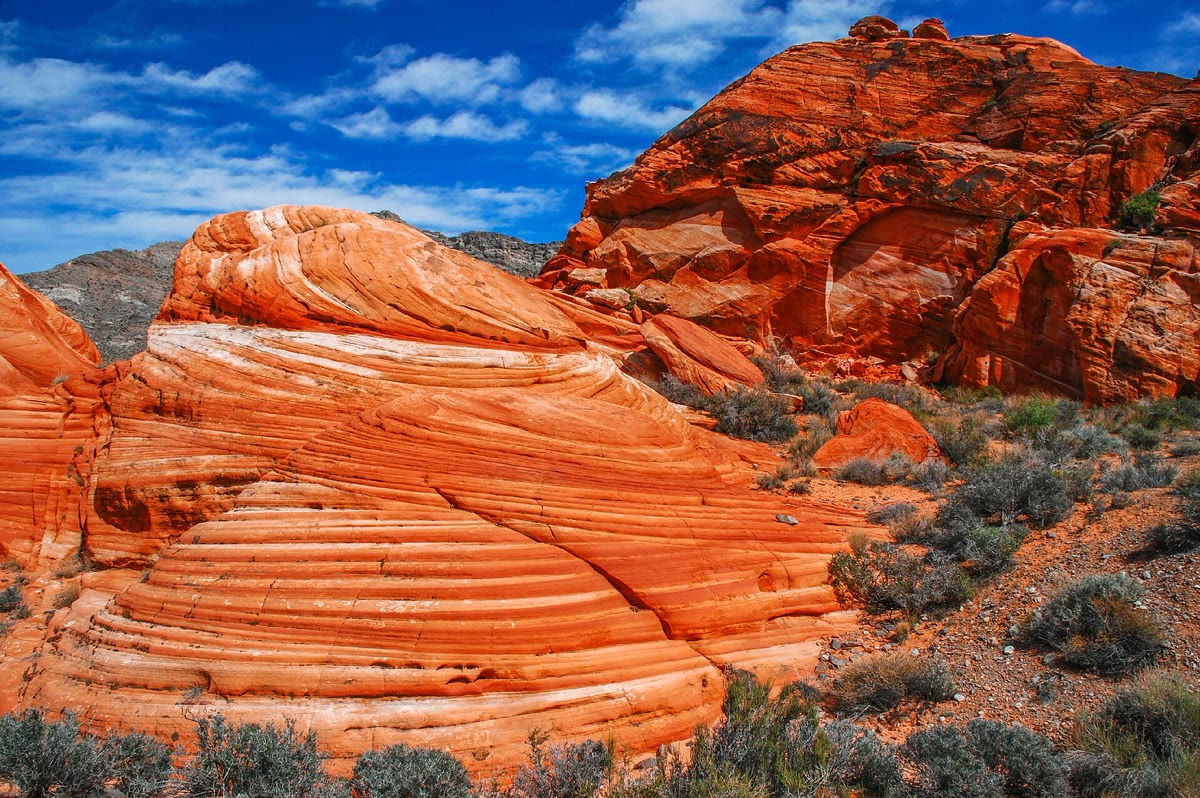
\includegraphics[height=3.6cm]{images/book3/b1-cross-bedding-aztec.jpg}};
\end{tikzpicture}

{\small À esquerda: a geometria das \omterm{def:b1:clastic-sediments:bedform}{formas de leito} em escalada (esquemático, ângulos exagerados). As calhas percorrem caminhos retos inclinados no ângulo de subida $\theta$ (linhas grossas); entre duas delas são preservadas as partes inferiores dos foresets, em conjuntos de espessura $T = L\sin\theta$. À direita: \omterm{def:b1:clastic-sediments:cross-bedding}{estratificação cruzada} no Arenito Aztec, Muddy Mountains, Nevada: conjuntos inclinados de lâminas, cada um cortado no topo pela superfície de erosão na base do seguinte. Fotografia de Chip Carroon, Bureau of Land Management, CC~BY-SA~2.0, via Wikimedia Commons.}
\label{fig:b1:clastic-sediments:climb}
\end{omfigure}
% ledger: southard:climb, commons:aztec-crossbed

\emph{\omterm{def:b1:clastic-sediments:cross-bedding}{Paleocorrentes}.} As direções de \omterm{def:b1:geological-maps:attitude}{mergulho} das estratificações cruzadas medidas num \omterm{def:b1:geological-maps:geological-map}{afloramento} se espalham em torno da \omterm{def:b1:geological-maps:attitude}{direção} média da corrente, pois as faces de sotavento de \omterm{def:b1:clastic-sediments:bedform}{dunas} e \omterm{def:b1:clastic-sediments:bedform}{marcas onduladas} são curvas, e as próprias correntes oscilam. Sua média é tomada como média vetorial, e não aritmética, pela razão mostrada em \cref{prop:b1:field-lab-methods-1:vector-mean}: \omterm{def:b1:spherical-astronomy:horizontal}{azimutes} são ângulos num círculo, e 350 e 010 têm média 000, não 180.

\begin{proposition}[Média de azimutes]\label{prop:b1:clastic-sediments:azimuths}
Sejam $\alpha_1, \ldots, \alpha_N$ \omterm{def:b1:spherical-astronomy:horizontal}{azimutes}, medidos no sentido horário a partir do norte. Sua média vetorial $\bar\alpha$ e seu comprimento médio resultante $\bar R$ são dados por
\[
  S = \sum_{i=1}^N \sin\alpha_i, \quad C = \sum_{i=1}^N \cos\alpha_i, \quad
  \bar\alpha = \operatorname{atan2}(S, C), \quad \bar R = \frac{\sqrt{S^2 + C^2}}{N},
\]
onde $\operatorname{atan2}(S, C)$ é o ângulo cujos seno e cosseno são proporcionais a $S$ e $C$, tomado entre \ang{0} e \ang{360}. $\bar R$ fica entre 0 e 1, e vale 1 apenas se todos os \omterm{def:b1:spherical-astronomy:horizontal}{azimutes} forem iguais.
\end{proposition}

\begin{proof}
O vetor unitário de \omterm{def:b1:spherical-astronomy:horizontal}{azimute} $\alpha$, com leste como primeira coordenada e norte como segunda, é $(\sin\alpha, \cos\alpha)$. A soma dos $N$ vetores unitários é $(S, C)$, e sua \omterm{def:b1:geological-maps:attitude}{direção}, a média vetorial (\cref{def:b1:field-lab-methods-1:mean-orientation}), tem o \omterm{def:b1:spherical-astronomy:horizontal}{azimute} cujos seno e cosseno são $S/\sqrt{S^2+C^2}$ e $C/\sqrt{S^2+C^2}$. Pela desigualdade triangular, o comprimento de uma soma de $N$ vetores unitários é no máximo $N$, com igualdade apenas quando todos apontam para o mesmo lado.
\end{proof}

\begin{method}[Paleocorrente a partir de estratificação cruzada]\label{met:b1:clastic-sediments:palaeocurrent}
\begin{enumerate}
  \item Em cada conjunto, meça a \omterm{def:b1:geological-maps:attitude}{direção} de \omterm{def:b1:geological-maps:attitude}{mergulho} dos foresets, escolhendo superfícies que mostrem seu verdadeiro \omterm{def:b1:geological-maps:attitude}{mergulho} (ou meça \omterm{def:b1:geological-maps:attitude}{direção} e \omterm{def:b1:geological-maps:attitude}{mergulho}).
  \item Meça a \omterm{def:b1:geological-maps:attitude}{atitude} do acamamento principal; se ele estiver inclinado em mais de alguns graus, gire cada foreset de volta à horizontal em torno da \omterm{def:b1:geological-maps:attitude}{direção} do acamamento (uma rotação feita com a projeção estereográfica do volume do Livro 5).
  \item Calcule a média vetorial $\bar\alpha$ e $\bar R$ das direções de \omterm{def:b1:geological-maps:attitude}{mergulho} corrigidas (\cref{prop:b1:clastic-sediments:azimuths}).
  \item Plote as leituras como um diagrama de rosa, um histograma circular de \omterm{def:b1:spherical-astronomy:horizontal}{azimutes}, para ver se elas formam um grupo ou dois: correntes de maré que se invertem constroem conjuntos com \omterm{def:b1:geological-maps:attitude}{mergulhos} em sentidos opostos, na \omterm{def:b1:clastic-sediments:cross-bedding}{estratificação cruzada} em espinha de peixe, e uma média única então não tem sentido.
\end{enumerate}
\end{method}
% ledger: og:sorting-environments

\emph{Outras estruturas.} Várias outras estruturas registram as condições de deposição e o lado para cima das camadas. Uma \omterm{def:b1:clastic-sediments:turbidite}{camada gradada} afina para cima, de grossa na base a fina no topo, à medida que os grãos se depositam de uma corrente em declínio, primeiro os mais grossos (\cref{def:b1:clastic-sediments:turbidite}). Fendas de ressecamento, polígonos de fendas de retração preenchidos pela camada seguinte, formam-se onde a lama seca ao ar, como em planícies de maré e de inundação. Escavações cortadas pela corrente na lama abaixo, e preenchidas pela areia de cima, se preservam como moldes na base do leito de arenito, e suas formas apontam para onde a corrente foi.
% ledger: og:sorting-environments

\section{Fácies, rios e deltas}\label{sec:b1:clastic-sediments:rivers-deltas}

A granulometria, a \omterm{def:b1:clastic-sediments:sorting}{seleção}, as estruturas, os fósseis e a composição juntos fazem o caráter de uma rocha sedimentar, e os geólogos usam uma só palavra para esse caráter.

\begin{definition}[Fácies sedimentar, ambiente de deposição]\label{def:b1:clastic-sediments:facies}
Uma \emph{fácies sedimentar}\index{fácies sedimentar} é um corpo de rocha sedimentar distinguido de outros por sua litologia, granulometria, estruturas sedimentares e fósseis, todos os quais refletem as condições em que foi formado. O \emph{ambiente de deposição}\index{ambiente de deposição} é o lugar, com suas condições físicas, químicas e biológicas, em que um sedimento é depositado: um canal de rio, uma planície de inundação, uma praia, o talude de um delta, o fundo do mar profundo.
\end{definition}
% ledger: og:sorting-environments

Uma fácies é uma descrição, um ambiente uma interpretação, e vários ambientes podem produzir a mesma fácies: areia com \omterm{def:b1:clastic-sediments:bedform}{marcas onduladas} é depositada em rios, em planícies de maré e no fundo do mar profundo. A interpretação repousa, portanto, em associações de fácies e na ordem em que se empilham, que seguem o movimento dos ambientes no espaço: as leis gerais desse empilhamento, e os modelos padrão de cada ambiente, são o assunto do volume do Livro 5. Este capítulo descreve os principais ambientes clásticos e as sucessões verticais que os identificam.

\emph{Rios entrelaçados e meandrantes.} Rios vêm em dois estilos principais. Um rio entrelaçado escoa em muitos canais que se dividem e se reencontram em torno de barras de cascalho e areia; rios entrelaçados carregam cargas grossas perto de suas nascentes, abaixo de montanhas ou à frente de geleiras, e seus depósitos são lençóis de cascalho e areia grossa com \omterm{def:b1:clastic-sediments:cross-bedding}{estratificação cruzada}, com pouca lama. Um rio meandrante escoa em um único canal sinuoso. A água mais rápida corre ao longo do lado de fora de cada curva, onde erode a margem escarpada; do lado de dentro, onde a água é mais lenta, deposita-se areia sobre a barra de ponta. O meandro assim migra de lado, erodindo de um lado e construindo do outro; a planície de inundação além das margens recebe apenas a lama das cheias.
% ledger: og:rivers

A sucessão da barra de ponta segue das \omterm{def:b1:clastic-sediments:bedform}{formas de leito}. No pé da barra, na água mais profunda e rápida, a corrente deixa os grãos mais grossos e constrói \omterm{def:b1:clastic-sediments:bedform}{dunas}; subindo a barra de declive suave a água se torna mais rasa e lenta, a areia mais fina, e as \omterm{def:b1:clastic-sediments:bedform}{dunas} cedem lugar a \omterm{def:b1:clastic-sediments:bedform}{marcas onduladas} (\cref{sec:b1:clastic-sediments:bedforms}); no topo, a barra passa à planície de inundação. À medida que a curva migra, cada uma dessas zonas se move sobre a que está abaixo, e um furo de sondagem através do depósito as encontra empilhadas: uma sucessão que afina para cima, de uma superfície de erosão até a lama, uma para cada passagem de um canal,
cuja espessura é cerca da profundidade do canal que o fez.

\emph{Deltas.} Onde um rio entra num corpo de água parado, sua corrente se espalha e desacelera, e sua carga se deposita: a carga grossa perto da foz, a fina mais longe. Um delta cresce para frente, ou prograda, enquanto o rio fornecer mais sedimento do que as ondas e as marés conseguem levar embora. O que as ondas e as marés fazem com esse aporte decide sua forma.

\begin{definition}[Deltas dominados por rios, por ondas e por marés]\label{def:b1:clastic-sediments:delta}
Um delta é \emph{dominado por rios}\index{delta dominado por rios} quando o aporte do rio sobrepuja as ondas e as marés, e seus canais distributários, confinados por seus próprios diques marginais, constroem longos dedos de areia no mar; é \emph{dominado por ondas}\index{delta dominado por ondas} quando as ondas retrabalham a areia trazida às fozes em praias e cordões de praia ao longo de uma costa lisa e arqueada; é \emph{dominado por marés}\index{delta dominado por marés} quando as correntes de maré, entrando e saindo das fozes, moldam sua areia em barras e cristas paralelas ao fluxo, separadas por canais em forma de funil.
\end{definition}
% ledger: og:deltas

\begin{omfigure}
\begin{tikzpicture}[font=\footnotesize, >={Stealth[length=4pt]}]
% meander in plan view (schematic) and the fining-upward log of a point bar
\begin{scope}[yscale=0.8]
  \fill[green!8] (-0.2,-0.4) rectangle (7.2,4.4);
  \draw[omSea!80!black, line width=9pt] plot[smooth, tension=0.7] coordinates {(0,3.6) (1.4,3.7) (2.6,2.8) (2.3,1.4) (3.2,0.5) (4.6,0.8) (5.0,2.2) (5.6,3.4) (7.0,3.5)};
  \draw[omSea!45, line width=7pt] plot[smooth, tension=0.7] coordinates {(0,3.6) (1.4,3.7) (2.6,2.8) (2.3,1.4) (3.2,0.5) (4.6,0.8) (5.0,2.2) (5.6,3.4) (7.0,3.5)};
  % point bars (inside of bends) with scroll lines
  \foreach \r in {0.25,0.45,0.65} {\draw[brown!60!black, densely dotted] (3.45,1.15) ++(200:\r) arc[start angle=200, end angle=340, radius=\r];}
  \fill[brown!25, opacity=0.8] (3.45,1.25) ellipse[x radius=0.55, y radius=0.35];
  \node[align=center] at (3.45,1.95) {barra de ponta\\ (deposição)};
  \fill[brown!25, opacity=0.8] (1.75,2.75) ellipse[x radius=0.4, y radius=0.45];
  \node[align=center] at (1.3,1.95) {barra de ponta};
  \draw[red!60!black, thick] (2.9,0.2) .. controls (3.3,0.0) and (4.3,0.15) .. (4.85,0.6);
  \node[red!60!black, anchor=north] at (4.0,0.0) {margem escarpada (erosão)};
  \draw[->, black!70] (5.9,3.0) -- (6.7,3.15) node[right] {escoamento};
  \node[anchor=north west, black!60] at (5.2,1.3) {planície de inundação};
  \node[font=\footnotesize] at (3.5,-0.85) {(a) um meandro, em planta};
\end{scope}
\begin{scope}[xshift=9.2cm, yshift=-0.3cm, yscale=0.8]
  % log: x width = grain size; y = height
  \draw[lith shale] (0,3.6) rectangle (0.8,4.6);
  \draw[lith sandstone] (0,2.6) rectangle (1.2,3.6);
  \draw[lith sandstone] (0,0.6) rectangle (1.7,2.6);
  \draw[lith conglomerate] (0,0) rectangle (2.2,0.6);
  \draw[very thick, red!60!black] (0,0) -- (2.2,0);
  % cross-bed symbols
  \foreach \y in {0.9,1.5,2.1} {\draw[black!70] (0.3,\y) .. controls (0.6,\y+0.05) and (0.9,\y+0.25) .. (1.2,\y+0.4);}
  \foreach \x in {0.2,0.5,0.8} {\draw[black!70] (\x,3.0) -- ++(0.12,0.1) -- ++(0.12,-0.1);}
  \node[anchor=west, align=left] at (2.4,4.1) {lama de planície,\\ raízes, fendas de ressecamento};
  \node[anchor=west, align=left] at (2.4,3.1) {areia fina, laminação\\ cruzada de marcas onduladas};
  \node[anchor=west, align=left] at (2.4,1.6) {areia média a grossa,\\ estratificação cruzada de dunas};
  \node[anchor=west, align=left] at (2.4,0.3) {resíduo de cascalho numa\\ superfície de erosão};
  \draw[->] (-0.35,0) -- (-0.35,4.6) node[above] {para cima};
  \draw[<->, black!60] (-0.7,0) -- node[above, rotate=90, font=\scriptsize] {profundidade do canal} (-0.7,3.6);
  \node[font=\footnotesize] at (1.8,-0.5) {(b) sucessão da barra de ponta};
\end{scope}
\end{tikzpicture}

{\small (a)~Um rio meandrante (esquemático): a corrente erode a margem externa de cada curva e deposita areia na barra de ponta do lado de dentro; as linhas curvas de deslocamento são as posições sucessivas da barra. (b)~A sucessão deixada por uma barra de ponta em migração, a largura de cada camada proporcional ao seu tamanho de grão (esquemático). Ela afina para cima, e sua espessura registra a profundidade do canal.}
\label{fig:b1:clastic-sediments:point-bar}
\end{omfigure}
% ledger: og:rivers, southard:phase-diagram

As três categorias extremas são os cantos de um triângulo no qual qualquer delta pode ser situado pela força relativa dos três processos. O delta em pé de pássaro do Mississippi, com seus longos dedos no golfo do México (\cref{ch:b1:erosion-transport}), é o clássico \omterm{def:b1:clastic-sediments:delta}{dominado por rios}; o Nilo, com seu arco liso de praias, um \omterm{def:b1:clastic-sediments:delta}{dominado por ondas}; o delta do Ganges e do Brahmaputra, o maior do mundo, um \omterm{def:b1:clastic-sediments:delta}{dominado por marés}.
% ledger: og:deltas

\begin{omfigure}
\begin{tikzpicture}[font=\footnotesize]
% delta classification triangle (schematic) and the Lena delta from Landsat
\begin{scope}[yscale=0.82]
  \coordinate (R) at (2.6,4.5); \coordinate (W) at (0,0); \coordinate (T) at (5.2,0);
  \fill[omDef!8] (R) -- (W) -- (T) -- cycle;
  \draw[thick] (R) -- (W) -- (T) -- cycle;
  \node[above, align=center] at (R) {\textbf{dominado por rios}\\ dedos alongados, diques marginais};
  \node[below, align=center] at (W) {\textbf{dominado por ondas}\\ cordões de praia suaves};
  \node[below, align=center] at (T) {\textbf{dominado por marés}\\ barras paralelas ao fluxo};
  \fill[omThm] (2.6,2.9) circle[radius=2pt] node[below=1pt] {Mississippi};
  \fill[omThm] (0.75,0.4) circle[radius=2pt] node[above right=0pt] {Nile};
  \fill[omThm] (4.4,0.4) circle[radius=2pt] node[above left=0pt, align=right] {Ganges--\\ Brahmaputra};
\end{scope}
\node[anchor=south west, inner sep=0] at (7.2,-0.9) {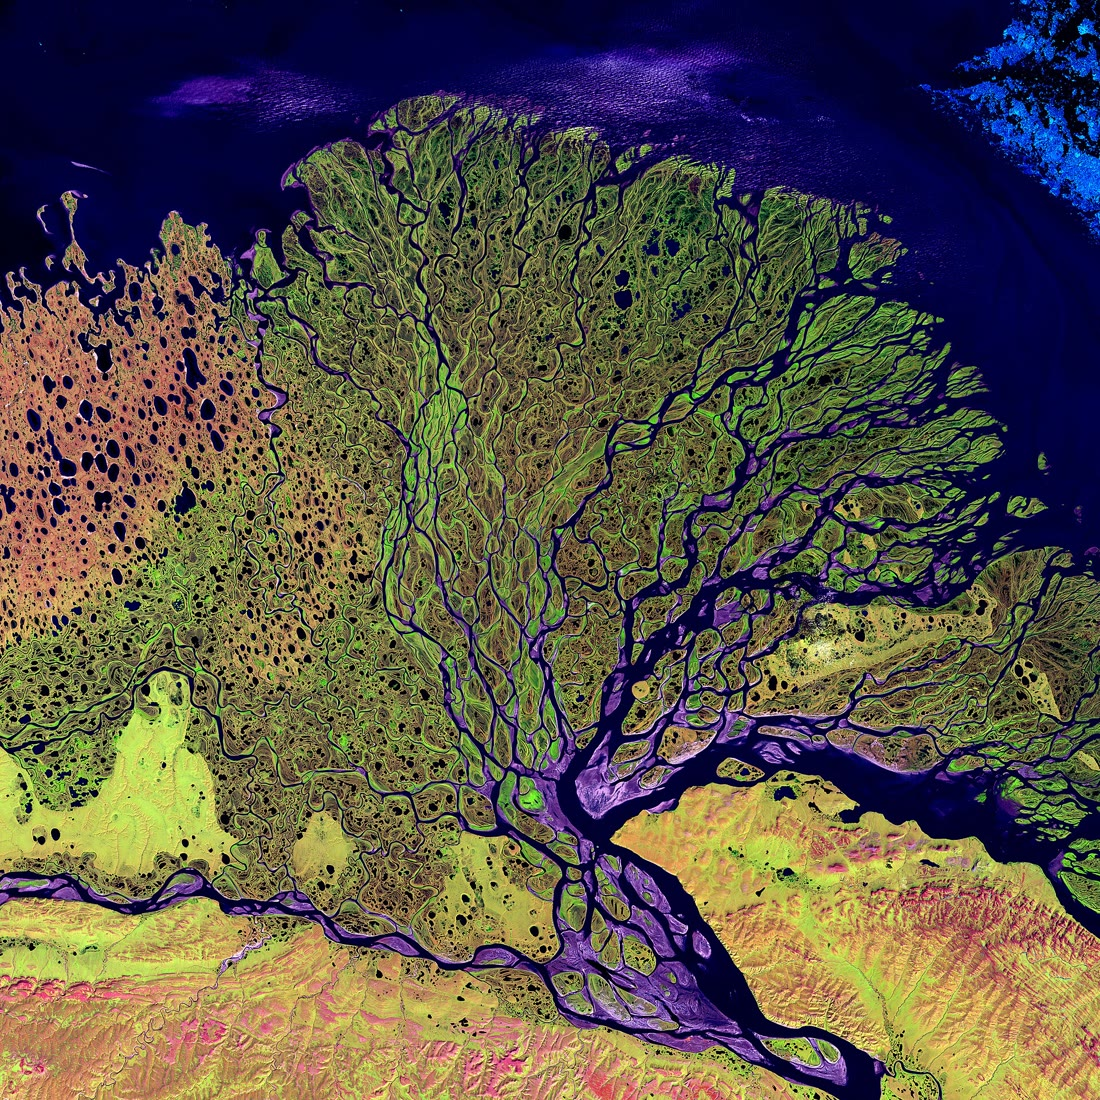
\includegraphics[height=5.2cm]{images/book3/b1-lena-delta.jpg}};
\end{tikzpicture}

{\small À esquerda: os três termos extremos dos deltas, segundo o processo que os molda (esquemático; as posições dos três exemplos são indicativas). À direita: o delta do Lena, na Sibéria, construído no mar de Laptev (no alto); o rio entra pelo canto inferior direito e se divide em centenas de distributárias. Imagem Landsat~7 em falsa cor de 27~de fevereiro de 2000, Serviço Geológico dos Estados Unidos, domínio público, via Wikimedia Commons.}
\label{fig:b1:clastic-sediments:deltas}
\end{omfigure}
% ledger: og:deltas, commons:lena-delta

\emph{A sucessão que engrossa para cima.} Em frente à foz do rio, o delta tem uma frente de declive suave, a frente deltaica, que passa para o mar adentro ao pró-delta, onde só a lama se deposita a partir da suspensão. À medida que o delta prograda, cada uma dessas zonas avança sobre a que está à sua frente: um furo de sondagem na planície deltaica encontra, de baixo para cima, as lamas laminadas do pró-delta, depois siltes e areias alternados da frente deltaica inferior, depois a areia com \omterm{def:b1:clastic-sediments:cross-bedding}{estratificação cruzada} das barras de foz, cortada no topo pelos canais da planície deltaica. A sucessão engrossa para cima, o inverso de uma barra de ponta, e sua espessura é cerca da profundidade da água em que o delta se construiu. Sua taxa está ligada à geometria da frente deltaica.

\begin{proposition}[Progradação e acumulação]\label{prop:b1:clastic-sediments:progradation}
Seja uma frente deltaica de declive constante $\alpha$ que avança horizontalmente à velocidade $v$ sem mudar de forma, com nível do mar constante. Um ponto fixo sob a frente recebe então sedimento à taxa vertical
\[
  a = v\,\tan\alpha,
\]
e a sucessão de frente deltaica de espessura $h$ se acumula ali no tempo $h/(v\tan\alpha)$.
\end{proposition}

\begin{proof}
No tempo $\mathrm dt$ a frente avança $v\,\mathrm dt$ à frente. Num ponto fixo sob a superfície inclinada, a superfície sobe pela diferença de altura entre dois pontos da frente separados horizontalmente por $v\,\mathrm dt$, isto é, $v\,\mathrm dt\,\tan\alpha$, daí a taxa. A frente atravessa o ponto enquanto a superfície sobe $h$, o que leva o tempo $h/a$.
\end{proof}

As frentes deltaicas têm declive suave, de modo que $\tan\alpha$ é pequeno: a frente de um delta avança muito mais depressa que o sedimento se acumula em qualquer ponto sob ela (\cref{exo:b1:clastic-sediments:12}).

\begin{inthelab}[Descrevendo um testemunho]
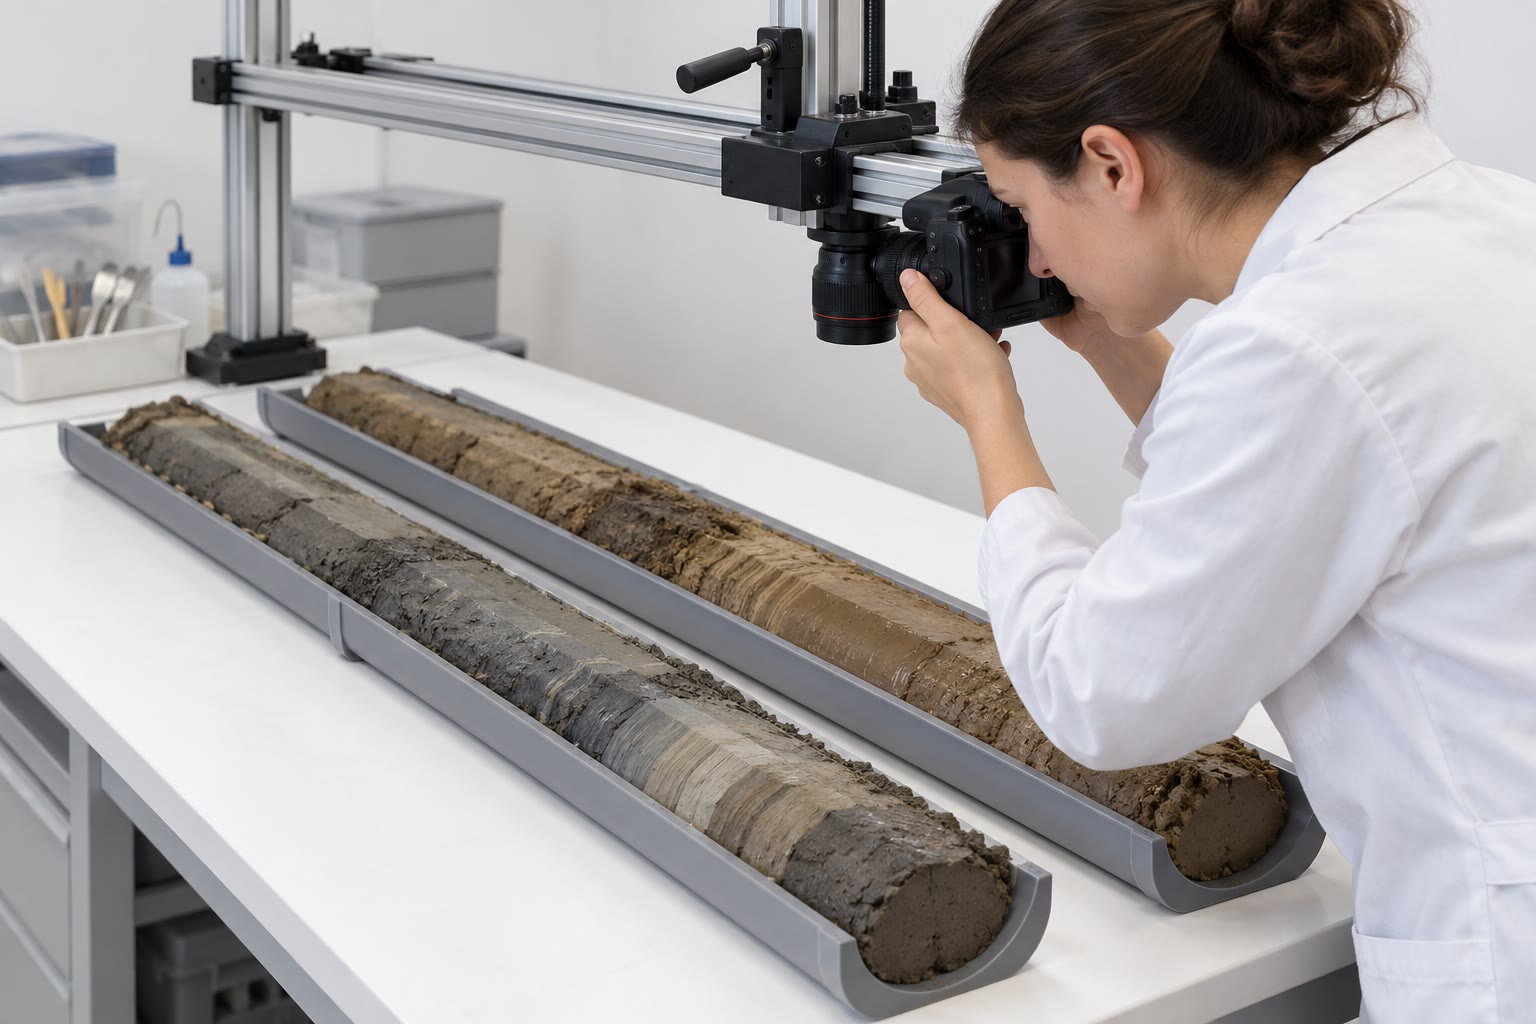
\includegraphics[width=0.3\linewidth]{images/book3/ai/b1-core-lab.jpg}\hfill
\begin{minipage}[b]{0.67\linewidth}
Os cilindros de sedimento ou rocha trazidos por uma sonda são dispostos em bandejas na ordem da profundidade, partidos ao longo e fotografados sob luz uniforme antes de secarem e mudarem de cor. O sedimentólogo então desenha um perfil do testemunho, metro a metro: a litologia, o tamanho de grão de cada camada (a largura da coluna), as estruturas (\omterm{def:b1:clastic-sediments:cross-bedding}{estratificação cruzada}, laminação, gradação, galerias), os \omterm{def:b1:geological-maps:geological-map}{contatos}, nítidos ou graduais, a cor e os fósseis. Amostras são retiradas para análise granulométrica e \omterm{def:b1:field-lab-methods-1:thin-section}{lâminas delgadas}. Um testemunho é uma janela estreita única: a \omterm{def:b1:geological-maps:attitude}{direção} das estratificações cruzadas se perde a menos que o testemunho tenha sido orientado, e a extensão lateral das camadas precisa vir de outras sondagens.
\end{minipage}

\smallskip
{\small Um testemunho disposto para ser fotografado em um laboratório de sedimentos (ilustração por IA).}
\end{inthelab}

\section{Litoral e plataforma}\label{sec:b1:clastic-sediments:shoreline}

Ao longo da costa entre os deltas, a areia trazida pelos rios é moldada por ondas e marés. Uma praia é areia retrabalhada pelo espraiamento, a fina lâmina de água que sobe e desce por ela depois que cada onda arrebenta: os grãos são movidos de novo e de novo, os finos são levados para o largo, e as areias de praia estão entre os sedimentos mais bem selecionados e mais arredondados de todos. Suas lâminas, depositadas pelo espraiamento, mergulham suavemente para o mar. Em muitas costas baixas a areia forma ilhas-barreira, cordões longos de praia e \omterm{def:b1:clastic-sediments:bedform}{dunas} eólicas separados do continente por lagunas, que são calmas e de granulação fina, ligadas ao mar por canais de maré.

Onde as marés são fortes e as ondas fracas, a costa é orlada por planícies de maré, cobertas e descobertas duas vezes por dia. Elas vão de areia perto da linha de maré baixa, onde as correntes são mais fortes, a lama perto da linha de maré alta, onde a água parada deixa a argila se depositar; seus depósitos mostram o escoamento que se inverte na \omterm{def:b1:clastic-sediments:cross-bedding}{estratificação cruzada} em espinha de peixe, o ressecamento em fendas de lama, e a alternância de corrente e água parada em finas camadas drapeadas de lama sobre areia com \omterm{def:b1:clastic-sediments:bedform}{marcas onduladas}.

Ao largo, a plataforma só é varrida pelas ondas até uma profundidade que cresce com o tamanho das ondas. Acima dela a areia é selecionada e movida; abaixo, a lama se deposita, exceto durante tempestades, quando as ondas maiores atingem mais fundo e depositam lençóis de areia com a laminação ondulada suave chamada \omterm{def:b1:clastic-sediments:cross-bedding}{estratificação cruzada} hummocky. Uma sucessão de plataforma assim alterna frequentemente lama de tempo bom com areias de tempestade, mais espessas e grossas em direção à costa.
% ledger: og:sorting-environments, folk:maturity

\section{Clásticos de mar profundo}\label{sec:b1:clastic-sediments:deep-sea}

Areia e cascalho também chegam ao fundo dos oceanos profundos, milhares de metros abaixo e centenas de quilômetros da terra, e são levados até lá por escoamentos que ninguém viu por inteiro: correntes densas e carregadas de sedimento que descem o talude continental sob a água limpa do oceano.

\begin{history}[Cabos no fundo do mar, 1929]
Em 18~de novembro de 1929 um terremoto de \omterm{def:b1:earthquake-source:mw}{magnitude de momento} 7.2 atingiu o talude continental ao sul de Terra Nova, ao longo da borda sul dos Grandes Bancos. Um escorregamento de cerca de \qty{200}{km^3} de sedimento desceu o talude, e um tsunami matou 28 pessoas na costa de Terra Nova. Doze cabos telegráficos estendidos pelo fundo do mar se romperam, alguns em vários pontos. Os mais próximos do epicentro romperam de imediato; os outros, mais ao sul e mais fundos, romperam um após o outro nas horas seguintes, na ordem da distância ladeira abaixo. Em 1952, Bruce Heezen e Maurice Ewing, estudando os horários das rupturas, as explicaram: o escorregamento havia se transformado em uma
\omterm{def:b1:clastic-sediments:turbidite}{corrente de turbidez} que desceu o talude e se espalhou pela planície abissal por mais de 480 milhas, rompendo cada cabo ao passar. A partir dos tempos e distâncias, estimaram sua velocidade em cerca de 50 nós na elevação continental superior, onde o talude tem cerca de \qty{0.5}{\percent}, e ainda 12 nós no último cabo, cerca de 400 milhas de sua origem. Ao desacelerar, argumentaram, ela deve ter depositado um leito gradado sobre a planície, cada vez mais fino para cima.
\end{history}
% ledger: nrcan:grand-banks, he52:grand-banks

Cinquenta nós são \qty{25.7}{m.s^{-1}}, mais de \qty{90}{km.h^{-1}}, a velocidade de um carro numa estrada principal; 12 nós são \qty{6.2}{m.s^{-1}}; e 480 milhas são cerca de \qty{770}{km}. As rupturas também deram as primeiras velocidades medidas de um escoamento que só havia sido inferido de seus depósitos e de experimentos em tanques.
% ledger: he52:grand-banks

\begin{definition}[Corrente de turbidez, turbidito, camada gradada]\label{def:b1:clastic-sediments:turbidite}
Uma \emph{corrente de turbidez}\index{corrente de turbidez} é uma corrente de água tornada mais densa que a água em torno dela pelo sedimento que carrega em suspensão, que escoa talude abaixo sob essa água, com seus grãos mantidos em suspensão pela turbulência que o próprio movimento cria. Um \emph{turbidito}\index{turbidito} é o depósito de uma corrente de turbidez. Uma \emph{camada gradada}\index{camada gradada} é uma camada cujo tamanho de grão diminui da base ao topo.
\end{definition}
% ledger: og:sorting-environments, he52:grand-banks

Uma \omterm{def:b1:clastic-sediments:turbidite}{corrente de turbidez} se alimenta a si mesma: ela corre porque sua suspensão é pesada, e mantém sua suspensão porque corre. Num talude íngreme ela pode apanhar mais sedimento do leito, tornar-se mais densa e acelerar; na suave declividade da planície abissal ela desacelera, larga sua carga e morre.

\begin{proposition}[Velocidade de uma corrente de turbidez]\label{prop:b1:clastic-sediments:turbidity}
Uma \omterm{def:b1:clastic-sediments:turbidite}{corrente de turbidez} de espessura $h$ e densidade $\rho + \Delta\rho$ escoa em regime permanente talude abaixo, de declive $S$, sob água de densidade $\rho$. Se a resistência do leito e da água acima dele é $\tau = \rho\,C_f\,U^2$ por unidade de área, sendo $C_f$ um coeficiente de atrito adimensional, sua velocidade média é
\[
  U = \sqrt{\frac{\Delta\rho}{\rho}\,\frac{g\,h\,S}{C_f}} .
\]
\end{proposition}

\begin{proof}
O argumento é o do produto profundidade--declividade (\cref{prop:b1:erosion-transport:depth-slope}), com o peso substituído pelo peso em excesso. Uma coluna da corrente de área unitária pesa $(\rho +
\Delta\rho) g h$, e a água que ela desloca $\rho g h$: na água em torno, só o excesso $\Delta\rho\,g\,h$ a puxa talude abaixo, com a componente $\Delta\rho\,g\,h\,S$ ao longo dele. Em escoamento permanente isso equilibra a resistência $\rho C_f U^2$, daí $U^2 = (\Delta\rho/\rho)\,g\,h\,S/C_f$.
\end{proof}

A lei de resistência $\tau = \rho C_f U^2$, quadrática na velocidade, é a dos escoamentos turbulentos da hidráulica (os livros de física), e $C_f$ é achado por experimento. A fórmula negligencia a água que a corrente incorpora a si pela sua superfície superior, o que a dilui e a desacelera. Ela mostra o papel dos três fatores: uma corrente duas vezes mais espessa, ou duas vezes mais densa, ou num talude duas vezes mais íngreme, corre $\sqrt 2$ vez mais depressa. Uma suspensão que tenha a fração $c$ de seu volume como grãos de quartzo tem $\Delta\rho/\rho = 1.65\,c$ (\cref{sec:b1:erosion-transport:settling}), pequeno a menos que o escoamento seja muito concentrado; é aí que uma \omterm{def:b1:clastic-sediments:turbidite}{corrente de turbidez} difere de um rio, no qual todo o peso da água, e não um pequeno excesso, impulsiona o escoamento. Para correr a 50 nós de 1929 num talude de meio por cento, uma \omterm{def:b1:clastic-sediments:turbidite}{corrente de turbidez} precisa de um produto grande de espessura e excesso de densidade (\cref{exo:b1:clastic-sediments:11}).

\emph{A sequência de Bouma.} Em 1962, Arnold Bouma descreveu a ordem interna das camadas de arenito de sucessões antigas de mar profundo em cinco divisões, rotuladas de baixo para cima. A: areia maciça ou gradada, muitas vezes sobre uma base erosiva; B: areia com laminação paralela; C: areia fina com laminação cruzada de \omterm{def:b1:clastic-sediments:bedform}{marcas onduladas}, muitas vezes convoluta; D: silte laminado que passa a lama; E: lama. A ordem é lida como o registro de uma única corrente em declínio passando sobre um ponto: à medida que desacelera, ela larga primeiro seus grãos mais grossos em massa, depois constrói um leito plano superior, depois \omterm{def:b1:clastic-sediments:bedform}{marcas onduladas}, e então deixa o silte e a argila se depositarem. Sequências completas são raras: as divisões superiores são muitas vezes erodidas pela corrente seguinte, e longe da fonte, onde a corrente é fraca, as inferiores faltam.
% ledger: og:sorting-environments, shanmugam:bouma

\begin{omfigure}
\begin{tikzpicture}[font=\footnotesize]
% Bouma sequence: log (schematic) and a labelled photograph
\begin{scope}
  \draw[lith shale] (0,4.0) rectangle (0.7,4.8);
  \draw[lith shale] (0,3.3) rectangle (0.9,4.0);
  \draw[lith sandstone] (0,2.2) rectangle (1.3,3.3);
  \draw[lith sandstone] (0,1.2) rectangle (1.6,2.2);
  \draw[lith sandstone] (0,0) rectangle (2.0,1.2);
  \draw[very thick, red!60!black] (0,0) .. controls (0.6,-0.12) and (1.4,0.1) .. (2.0,0);
  \foreach \y in {1.4,1.6,1.8,2.0} {\draw[black!70] (0.1,\y) -- (1.5,\y);}
  \foreach \x in {0.15,0.5,0.85} {\draw[black!70] (\x,2.55) .. controls (\x+0.12,2.75) .. (\x+0.3,2.6);}
  \foreach \y in {3.45,3.6,3.75,3.9} {\draw[black!60] (0.1,\y) -- (0.8,\y);}
  \foreach \x/\y in {0.4/0.3, 0.9/0.5, 1.4/0.25, 0.6/0.8, 1.2/0.9} {\fill[black!60] (\x,\y) circle[radius=0.06];}
  \node[anchor=west] at (2.2,4.4) {E \quad lama};
  \node[anchor=west] at (2.2,3.65) {D \quad silte laminado a lama};
  \node[anchor=west] at (2.2,2.75) {C \quad laminação cruzada de marcas onduladas};
  \node[anchor=west] at (2.2,1.7) {B \quad laminação paralela};
  \node[anchor=west] at (2.2,0.6) {A \quad areia gradada};
  \node[anchor=west, red!60!black] at (2.2,-0.15) {base erosiva, marcas de sola};
  \draw[->] (-0.3,0) -- (-0.3,4.8) node[above] {para cima};
\end{scope}
\node[anchor=south west, inner sep=0] at (6.9,-0.3) {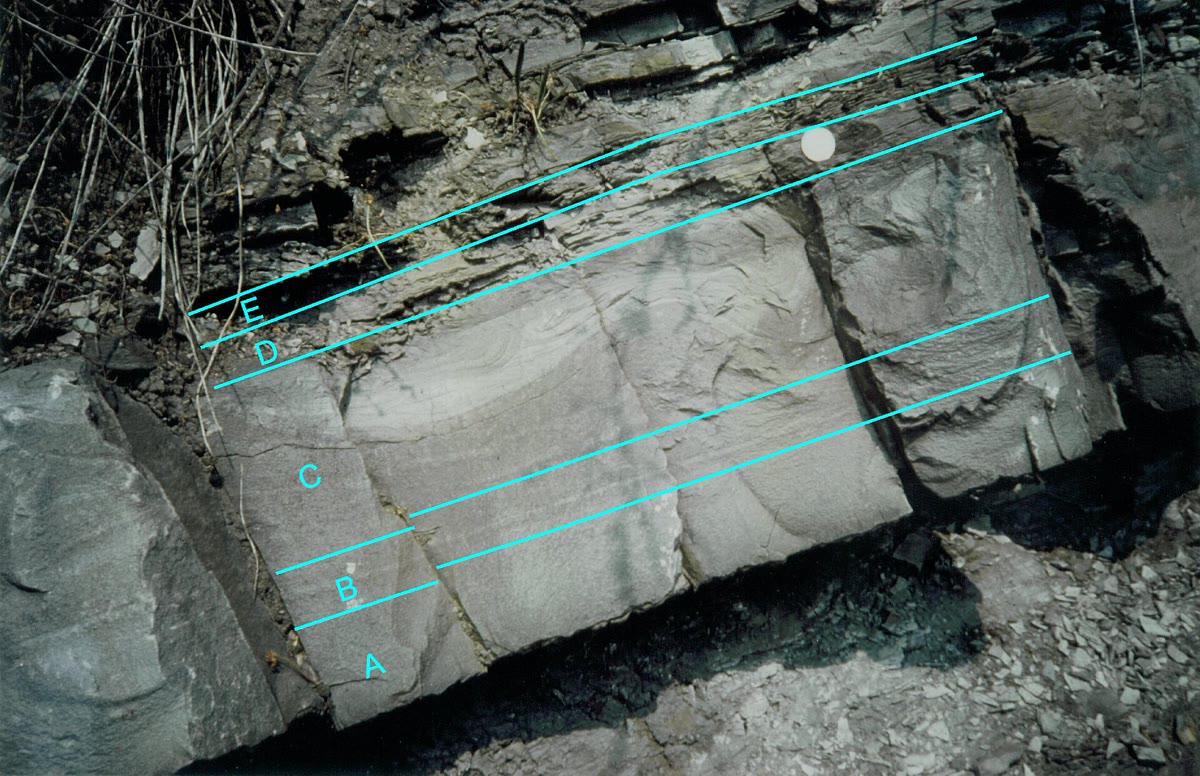
\includegraphics[height=5.2cm]{images/book3/b1-turbidite-bouma.jpg}};
\end{tikzpicture}

{\small À esquerda: as cinco divisões da sequência de Bouma, a largura de cada uma proporcional ao seu tamanho de grão (esquemático). À direita: uma camada de \omterm{def:b1:clastic-sediments:turbidite}{turbidito} do Devoniano Superior em Becke-Oese, Alemanha, com as divisões A a E marcadas pelo fotógrafo; a moeda dá a escala. Fotografia de Jo Weber, CC~BY-SA~3.0, via Wikimedia Commons.}
\label{fig:b1:clastic-sediments:bouma}
\end{omfigure}
% ledger: og:sorting-environments, shanmugam:bouma, commons:bouma-becke-oese

A sequência de Bouma tornou-se o modelo padrão do \omterm{def:b1:clastic-sediments:turbidite}{turbidito}, e milhares de arenitos antigos de mar profundo foram interpretados com ela. A interpretação é disputada: correntes que correm ao longo do talude, correntes profundas de maré e ondas internas também constroem areias com \omterm{def:b1:clastic-sediments:bedform}{marcas onduladas} e laminadas, e alguns sedimentólogos argumentam que muitas camadas lidas como \omterm{def:b1:clastic-sediments:turbidite}{turbiditos}, inclusive algumas da área-tipo, foram depositadas por outros escoamentos. Poucas \omterm{def:b1:clastic-sediments:turbidite}{correntes de turbidez} foram observadas no oceano atual, enquanto \omterm{def:b1:clastic-sediments:turbidite}{turbiditos} antigos são contados aos milhares.
% ledger: shanmugam:bouma

Nem todos os clásticos de mar profundo são \omterm{def:b1:clastic-sediments:turbidite}{turbiditos}. Correntes de contorno, as correntes lentas e profundas que seguem as curvas de nível do talude continental, retrabalham o sedimento do talude em derivas suaves e alongadas, os contoritos. E longe dos continentes, onde nem \omterm{def:b1:clastic-sediments:turbidite}{correntes de turbidez} nem correntes de contorno chegam, o fundo do mar recebe apenas o que se deposita da água acima: as conchas do plâncton e a poeira eólica mais fina, os sedimentos pelágicos do próximo capítulo (\cref{ch:b1:chemical-biogenic-sediments}).
% ledger: og:sorting-environments

\section{Exercícios}

\begin{exercise}[$\star$]\label{exo:b1:clastic-sediments:1}
Converta em unidades phi os diâmetros \qty{0.18}{mm}, \qty{0.75}{mm}, \qty{3}{mm}, \qty{0.012}{mm} e \qty{150}{mm}, com duas casas decimais, e dê a classe de cada um (\cref{tab:b1:clastic-sediments:classes}).
% ledger: folk:wentworth-classes
\end{exercise}

\begin{exercise}[$\star$]\label{exo:b1:clastic-sediments:2}
A curva acumulada de uma areia de rio dá $\varphi_5 = 0.62$, $\varphi_{16} =
1.05$, $\varphi_{50} = 1.71$, $\varphi_{84} = 2.43$ e $\varphi_{95} = 2.98$. Calcule sua média gráfica, em unidades phi e em milímetros, e seu desvio-padrão gráfico inclusivo, e dê o nome de seu tamanho e de sua \omterm{def:b1:clastic-sediments:sorting}{seleção}.
% ledger: folk:graphic-measures, folk:sorting-classes
\end{exercise}

\begin{exercise}[$\star$]\label{exo:b1:clastic-sediments:3}
\omterm{def:b1:clastic-sediments:bedform}{Marcas onduladas} de \qty{2}{cm} de altura migram a \qty{1}{cm} por minuto sobre um leito de areia de quartzo de porosidade \num{0.4}. Com \cref{prop:b1:clastic-sediments:migration}, calcule o volume de \omterm{def:b1:erosion-transport:load}{carga de fundo} por unidade de largura, em \si{m^2.s^{-1}}, e a massa de quartzo ($\qty{2650}{kg.m^{-3}}$) transportada sobre um metro de crista em um dia.
% ledger: hom:quartz
\end{exercise}

\begin{exercise}[$\star$]\label{exo:b1:clastic-sediments:4}
Um nó é uma milha náutica, \qty{1852}{m}, por hora. (a)~Converta em metros por segundo as velocidades de 50 e 12 nós estimadas para a \omterm{def:b1:clastic-sediments:turbidite}{corrente de turbidez} de 1929. (b)~Quanto tempo uma corrente a 12 nós leva para percorrer \qty{100}{km}? (c)~Converta 480 e 400 milhas em quilômetros (uma milha tem \qty{1.609}{km}).
% ledger: he52:grand-banks
\end{exercise}

\begin{exercise}[$\star\star$]\label{exo:b1:clastic-sediments:5}
(a)~Usando os percentis de uma distribuição normal dados na demonstração de \cref{prop:b1:clastic-sediments:normal}, calcule o desvio-padrão gráfico $(\varphi_{84} - \varphi_{16})/2$ e a estimativa $(\varphi_{95} - \varphi_5)/3.3$ para uma distribuição normal de desvio-padrão $\sigma$. (b)~Por que as duas podem discordar para um sedimento real? Que tipo de sedimento as faz diferir mais?
\end{exercise}

\begin{exercise}[$\star\star$]\label{exo:b1:clastic-sediments:6}
Um depósito de \omterm{def:b1:clastic-sediments:bedform}{marcas onduladas} em escalada mostra conjuntos de \qty{1.5}{cm} de espessura, medida perpendicularmente a seus limites, feitos por \omterm{def:b1:clastic-sediments:bedform}{marcas onduladas} espaçadas de \qty{15}{cm}. (a)~Calcule o ângulo de subida. (b)~Se as marcas se moveram a \qty{0.5}{cm} por minuto, a que taxa o leito foi elevado, em centímetros por hora? (c)~O que uma taxa assim diz sobre o escoamento?
% ledger: southard:climb
\end{exercise}

\begin{exercise}[$\star\star$]\label{exo:b1:clastic-sediments:7}
Seis direções de \omterm{def:b1:geological-maps:attitude}{mergulho} de \omterm{def:b1:clastic-sediments:cross-bedding}{estratificação cruzada}, já corrigidas pela inclinação das camadas, dão 350, 020, 005, 340, 015 e 030. (a)~Calcule sua média aritmética. (b)~Calcule sua média vetorial e $\bar R$. (c)~Explique a diferença.
\end{exercise}

\begin{exercise}[$\star\star$]\label{exo:b1:clastic-sediments:8}
Três arenitos são examinados em \omterm{def:b1:field-lab-methods-1:thin-section}{lâmina delgada}. A tem \qty{12}{\percent} de matriz argilosa e grãos angulosos de quartzo, \omterm{def:b1:rock-forming-minerals:groups}{feldspato} e fragmentos de rocha. B tem \qty{2}{\percent} de argila, $\sigma_I = 0.40\,\varphi$ e grãos de quartzo de arredondamento \num{2.2} na escala de Folk. C não tem argila, $\sigma_I =
0.30\,\varphi$, grãos de quartzo de arredondamento \num{3.6}, e \qty{98}{\percent} de quartzo. Dê a \omterm{def:b1:clastic-sediments:maturity}{maturidade textural} de cada um e sugira um ambiente de deposição para cada.
% ledger: folk:maturity
\end{exercise}

\begin{exercise}[$\star\star$]\label{exo:b1:clastic-sediments:9}
(a)~Calcule o número de Froude de um escoamento de \qty{0.3}{m} de profundidade a \qty{1.5}{m.s^{-1}}, e de um rio de \qty{2}{m} de profundidade a \qty{1.0}{m.s^{-1}} ($g
= \qty{9.81}{m.s^{-2}}$). (b)~Em que profundidade um escoamento de \qty{1.5}{m.s^{-1}} atingiria um número de Froude de 1, e que velocidade o rio de \qty{2}{m} de profundidade precisaria ter? (c)~Por que antidunas são comuns em lâminas de água que correm
de uma praia, e raras em rios grandes?
% ledger: southard:ripples-dunes
\end{exercise}

\begin{exercise}[$\star\star\star$]\label{exo:b1:clastic-sediments:10}
Uma análise granulométrica de uma areia dá, em classes phi inteiras de $-1$ a $5\,\varphi$: 2, 8, 30, 40, 15 e 5 por cento em peso. (a)~Pelo método dos momentos, calcule a média e o desvio-padrão em unidades phi, e dê o nome da \omterm{def:b1:clastic-sediments:sorting}{seleção}. (b)~Construa a curva acumulada, leia $\varphi_5$, $\varphi_{16}$, $\varphi_{50}$, $\varphi_{84}$ e $\varphi_{95}$ por interpolação linear, e calcule $M_z$ e $\sigma_I$. (c)~Compare.
% ledger: folk:graphic-measures, folk:sorting-classes
\end{exercise}

\begin{exercise}[$\star\star\star$]\label{exo:b1:clastic-sediments:11}
Tome $C_f = 0.003$ em \cref{prop:b1:clastic-sediments:turbidity}. (a)~Uma \omterm{def:b1:clastic-sediments:turbidite}{corrente de turbidez} de \qty{50}{m} de espessura, com excesso de densidade de \qty{2}{\percent}, desce um talude de \num{0.005}: calcule sua velocidade, em metros por segundo e em nós. (b)~Que produto de espessura e excesso relativo de densidade daria os 50 nós de 1929 no mesmo talude? (c)~A mesma corrente de (a) chega a um talude de \num{0.001}: calcule sua nova velocidade, se nada mais mudar. O que acontece com sua carga?
% ledger: he52:grand-banks
\end{exercise}

\begin{exercise}[$\star\star\star$]\label{exo:b1:clastic-sediments:12}
Um rio entrega \qty{50}{Mt} de sedimento por ano a seu delta, dos quais \qty{70}{\percent} se depositam numa frente deltaica de \qty{100}{km} de largura que se constrói numa água de \qty{30}{m} de profundidade. O depósito tem densidade aparente de \qty{2000}{kg.m^{-3}}. (a)~Que volume ele acrescenta por ano? (b)~Se esse volume preenche toda a profundidade da água ao longo da largura da frente, com que velocidade a frente avança? (c)~Com um declive da frente deltaica de \ang{0.5}, a que taxa o sedimento se acumula num ponto fixo sob a frente, e em quantos anos se forma ali a sucessão que engrossa para cima?
\end{exercise}

\section{Problema: lendo um testemunho de um delta}

\begin{problem}[{Problema de fim de semana --- uma sondagem através de um delta antigo, dos tamanhos de grão à direção de seus rios}]
\label{pb:b1:clastic-sediments:1}
% values: calc/ch21.py; the borehole, its beds, ages and readings are invented
Uma sondagem atravessa \qty{24}{m} de arenitos e lamitos depositados por um delta antigo. O geólogo descreve quatro unidades, da base para cima, e analisa uma amostra de cada uma.

\smallskip
\begin{center}\small
\begin{tabular}{@{}llccccc@{}}
\hline
unidade (prof. a partir da base) & descrição & $\varphi_5$ & $\varphi_{16}$ & $\varphi_{50}$ & $\varphi_{84}$ & $\varphi_{95}$ \\
\hline
1 (0--8 m) & lamito cinza laminado & 4.2 & 5.0 & 6.6 & 8.4 & 9.6 \\
2 (8--16 m) & siltito e arenito alternados & 1.9 & 2.4 & 3.4 & 4.6 & 5.5 \\
3 (16--21 m) & arenito com \omterm{def:b1:clastic-sediments:cross-bedding}{estratificação cruzada} & 0.9 & 1.25 & 1.8 & 2.35 & 2.7 \\
4 (21--24 m) & arenito com seixos, base erosiva & $-1.8$ & $-0.8$ & 0.9 & 2.1 & 2.9 \\
\hline
\end{tabular}
\end{center}

\medskip
\noindent\textbf{Parte I --- Os tamanhos de grão.}
\begin{enumerate}
  \item Calcule a média gráfica $M_z$ de cada unidade, em unidades phi e em milímetros.
  \item Calcule o desvio-padrão gráfico inclusivo $\sigma_I$ de cada unidade.
  \item Dê o nome da classe de tamanho da média e da \omterm{def:b1:clastic-sediments:sorting}{seleção} de cada unidade.
  \item Qual unidade é a mais bem selecionada? Por que uma barra de foz seria mais bem selecionada que as lamas do pró-delta?
  \item Interpolando linearmente entre $\varphi_{50}$ e $\varphi_{84}$, estime a porcentagem de partículas do tamanho de argila (mais finas que $8\,\varphi$) na unidade~1. O que isso diz sobre as correntes onde ela foi depositada?
  \item Por que a curva acumulada da unidade~4 é tão espalhada, embora seja uma areia de canal?
\end{enumerate}

\medskip
\noindent\textbf{Parte II --- A sucessão.}
\begin{enumerate}[resume]
  \item Descreva como o tamanho médio muda da unidade~1 à unidade~3. A sucessão afina ou engrossa para cima?
  \item Interprete as unidades 1, 2 e 3 como partes de um delta. Que zona do delta estava no local quando cada uma foi depositada?
  \item O que o empilhamento das três unidades mostra sobre o movimento do delta?
  \item Qual profundidade de água o delta construiu, no mínimo, e por quê?
  \item A unidade~4 tem base erosiva e é mais grossa que a unidade~3. Interprete-a.
  \item Uma barra de ponta daria a mesma sucessão? Explique.
\end{enumerate}

\medskip
\noindent\textbf{Parte III --- Com que rapidez o delta avançou?}
Duas camadas finas de cinza vulcânica, na base da unidade~1 e no topo da unidade~2, são datadas; estão separadas por \num{4000}~anos.
\begin{enumerate}[resume]
  \item Calcule a taxa média de acumulação entre as duas cinzas, em milímetros por ano.
  \item A frente deltaica tinha declive de \ang{0.5}. Com \cref{prop:b1:clastic-sediments:progradation}, calcule a velocidade com que ela avançou, em metros por ano.
  \item Quanto a frente avançou durante os \num{4000}~anos?
  \item Quanto tempo levaram os 21 metros das unidades 1 a 3 para se acumular no local, nessa taxa?
  \item Por que a taxa de acumulação num delta não é a mesma em toda parte, num mesmo tempo?
\end{enumerate}

\medskip
\noindent\textbf{Parte IV --- Para onde correram os rios?}
Sobre o arenito com \omterm{def:b1:clastic-sediments:cross-bedding}{estratificação cruzada} da unidade~3, exposto num \omterm{def:b1:geological-maps:geological-map}{afloramento} próximo onde o acamamento é horizontal, são medidas doze direções de \omterm{def:b1:geological-maps:attitude}{mergulho} dos foresets: 352, 010, 025, 004, 338, 017, 031, 359, 012, 046, 006 e 344.
\begin{enumerate}[resume]
  \item Calcule a média aritmética das doze leituras. Ela tem sentido?
  \item Calcule as somas $S$ e $C$ de \cref{prop:b1:clastic-sediments:azimuths}.
  \item Calcule o comprimento médio resultante $\bar R$. As leituras são consistentes?
  \item Em que direção geral o delta se construiu, e onde estava a terra?
  \item Por que as direções de \omterm{def:b1:geological-maps:attitude}{mergulho} devem ser giradas se as camadas estão inclinadas, e em torno de que eixo?
  \item Uma corrente de maré poderia ter construído essas estratificações cruzadas? Como seria seu diagrama de rosa?
  \item Com aproximação de um grau, qual é o \omterm{def:b1:spherical-astronomy:horizontal}{azimute} médio da \omterm{def:b1:clastic-sediments:cross-bedding}{paleocorrente} do arenito com \omterm{def:b1:clastic-sediments:cross-bedding}{estratificação cruzada} da unidade~3?
\end{enumerate}
\end{problem}
